% ====================================================================
% PLANTILLA INFORME PRIMERA ENTREGA - GEOINFORMÁTICA USACH
% Autor: Prof. Francisco Parra O.
% ====================================================================

\documentclass[11pt,letterpaper]{article}

% PAQUETES ESENCIALES
\usepackage[utf8]{inputenc}
\usepackage[spanish,es-tabla]{babel}
\usepackage[left=2.5cm,right=2.5cm,top=2.5cm,bottom=2.5cm]{geometry}
\usepackage{graphicx}
\usepackage{float}
\usepackage{xcolor}
\usepackage{hyperref}
\usepackage{amsmath,amssymb}
\usepackage{booktabs}
\usepackage{caption}
\usepackage{newunicodechar}
\newunicodechar{≥}{\geq}
\usepackage{subcaption}
\usepackage{longtable}
\usepackage{array}
\usepackage{multirow}
\usepackage{listings}
\usepackage{fancyhdr}
\usepackage{lastpage}
\usepackage[backend=biber,style=apa]{biblatex}

% Configuración de bibliografía
%\addbibresource{referencias.bib} % Crear este archivo para las referencias

% Colores institucionales
\definecolor{usachblue}{RGB}{0,46,93}
\definecolor{usachred}{RGB}{200,16,46}
\definecolor{codegreen}{rgb}{0,0.6,0}
\definecolor{codegray}{rgb}{0.5,0.5,0.5}
\definecolor{codepurple}{rgb}{0.58,0,0.82}
\definecolor{backcolour}{rgb}{0.95,0.95,0.92}

% Configuración de código
\lstdefinestyle{mystyle}{
    backgroundcolor=\color{backcolour},
    commentstyle=\color{codegreen},
    keywordstyle=\color{magenta},
    numberstyle=\tiny\color{codegray},
    stringstyle=\color{codepurple},
    basicstyle=\ttfamily\footnotesize,
    breakatwhitespace=false,
    breaklines=true,
    captionpos=b,
    keepspaces=true,
    numbers=left,
    numbersep=5pt,
    showspaces=false,
    showstringspaces=false,
    showtabs=false,
    tabsize=2,
    language=Python
}
\lstset{style=mystyle}

% Configuración de hyperref
\hypersetup{
    colorlinks=true,
    linkcolor=usachblue,
    filecolor=magenta,
    urlcolor=usachblue,
    citecolor=usachblue
}

% Encabezado y pie de página
\pagestyle{fancy}
\fancyhf{}
\lhead{\textcolor{usachblue}{Geoinformática - Primera Entrega}}
\rhead{\textcolor{usachblue}{USACH 2025}}
\lfoot{\small\textit{Terramatch}}
\cfoot{\thepage\ de \pageref{LastPage}}
\rfoot{\today}

% ====================================================================
% PORTADA - MODIFICAR CON SUS DATOS
% ====================================================================

\begin{document}

\begin{titlepage}
    \centering
    \vspace*{1cm}

    \Large{\textbf{UNIVERSIDAD DE SANTIAGO DE CHILE}}\\
    \large{Facultad de Ingeniería}\\
    \large{Departamento de Ingeniería Informática}\\

    \vspace{3cm}

    \rule{\textwidth}{0.5mm}\\
    \vspace{0.5cm}

    {\LARGE\textbf{TerraMatch}}\\
    \vspace{0.3cm}
    {\Large\textit{Sistema de estimación de satisfacción inmobiliaria basado en información geoespacial}}\\

    \vspace{0.5cm}
    \rule{\textwidth}{0.5mm}

    \vspace{2cm}

    {\Large\textbf{Primera Evaluación}}\\
    \vspace{0.5cm}
    {\large Informe de Avance}

    \vspace{3cm}

\begin{minipage}{0.8\textwidth}
    \begin{flushleft}
        \large
        \textbf{Integrantes del Grupo:}\\
        Valentina Del Pilar Barr\'ia - 21.149.435-2\\
        Felipe Baeza Mu\~noz - 20.637.464-0\\
        Byron Caices Lima - 20.915.795-0\\
        Catalina L\'opez - 21.051.116-4\\
        Jaime Antonio Riquelme Olguin - 20.964.708-7\\
        Diego Ignacio Rojas Bustos - 17.464.162-5\\
        \vspace{0.5cm}
        \textbf{Profesor:}\\
        Francisco Parra O.\\
        \vspace{0.5cm}
        \textbf{Ayudantes:}\\
        %[Si aplica]
    \end{flushleft}
\end{minipage}


    \vfill

    {\large \today}
\end{titlepage}

% ====================================================================
% RESUMEN EJECUTIVO
% ====================================================================

\newpage
\section*{Resumen Ejecutivo}
\addcontentsline{toc}{section}{Resumen Ejecutivo}
% [Máximo 1 página]
% Incluir: problema abordado, área de estudio, metodología principal,
% resultados preliminares clave, y próximos pasos.

El mercado inmobiliario chileno atraviesa una crisis de acceso a la vivienda caracterizada por el requisito de un 20\% de pie inicial para créditos hipotecarios, monto que representa aproximadamente 32 veces el ingreso mediano del país y que coloca a numerosos hogares en una situación donde no califican para créditos bancarios ni para subsidios estatales. Esta realidad ha generado consumidores cada vez más exigentes que buscan maximizar la satisfacción de su inversión inmobiliaria, demandando herramientas objetivas que les permitan evaluar propiedades más allá del precio. En este contexto, TerraMatch surge como un sistema de apoyo a la decisión que integra información geoespacial para estimar la satisfacción residencial potencial de propiedades en venta.

El proyecto se desarrolla sobre cuatro comunas de la Región Metropolitana de Santiago: Estación Central, La Reina, Ñuñoa y Santiago Centro. Esta selección responde a criterios de diversidad socioeconómica (desde estratos altos en La Reina hasta medios-bajos en Estación Central), heterogeneidad urbana (zonas de alta densificación vertical versus sectores residenciales tradicionales) y disponibilidad de datos suficientes para el entrenamiento de modelos predictivos.

La metodología implementada comprende cinco etapas: extracción automatizada de 7.702 propiedades mediante web scraping de Portal Inmobiliario, geocodificación de direcciones utilizando Google Maps API en el sistema de coordenadas EPSG:32719 (UTM Zone 19S), cálculo de 42 variables espaciales mediante distancias euclidianas a puntos de interés (estaciones de metro, centros educacionales, de salud, seguridad, comercio y áreas verdes), diseño de un índice de satisfacción residencial como variable objetivo, y entrenamiento de modelos predictivos mediante Machine Learning.

Los resultados preliminares demuestran que el modelo exploratorio híbrido GWRF por cluster explica el 88\% de la varianza observada con un error medio absoluto de 439 UF/m². Tras una comparación exhaustiva de algoritmos, el modelo LightGBM fue seleccionado como modelo final, alcanzando un R² de 0.8635 con RMSE de 0.3357 y baja autocorrelación espacial de residuos (Moran's I = 0.0695), lo que indica ausencia de sesgo geográfico en las predicciones. Las próximas fases contemplan la expansión geográfica a comunas adicionales, incorporación de variables temporales, desarrollo de API REST para predicciones en tiempo real, implementación de interfaz web interactiva, y validación mediante encuestas de satisfacción real de usuarios.

% ====================================================================
% ÍNDICE
% ====================================================================

\newpage
\tableofcontents
\newpage

% ====================================================================
% 1. INTRODUCCIÓN
% ====================================================================

\section{Introducción}

\subsection{Contexto y Motivación}
El mercado inmobiliario chileno enfrenta una barrera de acceso relevante: el pie hipotecario del 20\% equivale a ~32 veces el ingreso mediano, lo que excluye a muchos hogares de credito y subsidios. Entre 2021 y 2023 la demanda de viviendas se contrajo, con caidas en ventas y mayores desistimientos, y en 2025 se observo un stock cercano a 70.000 unidades, abriendo oportunidades para compradores \cite{biobio_ciper_2025}. El estudio IPSOS 2025 muestra brechas de satisfaccion entre propietarios (74\%) y arrendatarios (39\%) \cite{ipsos_monitor_2025}, reforzando la necesidad de herramientas objetivas para comparar alternativas.

Ademas de la contraccion de la demanda, las restricciones crediticias y el aumento del costo de la construccion han reducido la accesibilidad a la vivienda. Para muchos hogares, comparar alternativas requiere mirar mas alla del precio y considerar conectividad, acceso a servicios y calidad del entorno. Un enfoque geoespacial permite cuantificar estas condiciones de forma objetiva y comparable entre barrios.

Los factores de decision mas frecuentes combinan precio, seguridad, accesibilidad y entorno urbano. TerraMatch propone integrar datos geoespaciales para estimar satisfaccion residencial potencial y apoyar decisiones de compra con criterios medibles. Entre los criterios mas mencionados se consideran:

\begin{itemize}
    \item Relacion precio/m\textsuperscript{2} y costo total de la propiedad.
    \item Seguridad y presencia de servicios de emergencia cercanos.
    \item Acceso a transporte publico y conectividad urbana.
    \item Proximidad a educacion, salud y comercio.
    \item Acceso a areas verdes y espacios recreativos.
    \item Condiciones de habitabilidad (tamano, distribucion, privacidad).
\end{itemize}

La propuesta busca reducir la asimetria de informacion y entregar una evaluacion comparable entre comunas y perfiles de usuario.

\subsection{Objetivos}

\subsubsection{Objetivo General}
Desarrollar un sistema de recomendacion inmobiliaria que prediga la satisfaccion residencial integrando atributos internos de la vivienda con variables geoespaciales del entorno urbano, usando Machine Learning (LightGBM) para apoyar decisiones de compra en la Region Metropolitana de Santiago.

\subsubsection{Objetivos Específicos}
\begin{enumerate}
    \item Integrar y normalizar 29 datasets geoespaciales en EPSG:32719, con control de calidad y trazabilidad.
    \item Calcular metricas espaciales (distancias, densidades e indices) y asociarlas a 7,702 propiedades geocodificadas.
    \item Disenar un proxy de satisfaccion residencial y perfiles de usuario para ponderar preferencias.
    \item Entrenar y validar un modelo predictivo (LightGBM) con evaluacion comparativa y metricas robustas.
    \item Generar visualizaciones y un prototipo de recomendacion (API/mapa interactivo) para explorar resultados.
\end{enumerate}

\subsection{Preguntas de Investigación}

\subsubsection{Pregunta Principal}
\textbf{¿Que hace que una vivienda sea satisfactoria para vivir en el contexto urbano de Santiago?}

\subsubsection{Preguntas Secundarias}
\begin{itemize}
    \item ¿Que peso tienen los factores espaciales (acceso a servicios, transporte y areas verdes) respecto al precio y atributos internos?
    \item ¿Existen patrones territoriales y diferencias entre comunas en la satisfaccion predicha?
    \item ¿Como cambian los determinantes de satisfaccion segun el perfil de usuario?
\end{itemize}

\subsubsection{Hipótesis de Trabajo}
\begin{itemize}
    \item \textbf{H1}: Los factores espaciales externos influyen significativamente en la satisfaccion residencial.
    \item \textbf{H2}: Existe autocorrelacion espacial positiva en la satisfaccion residencial.
    \item \textbf{H3}: Los determinantes de satisfaccion varian segun el perfil de usuario.
    \item \textbf{H4}: Incorporar variables geoespaciales mejora la capacidad predictiva frente a modelos solo con atributos internos.
\end{itemize}

\subsection{Alcance y Limitaciones}
\textbf{Alcance geografico:} Cuatro comunas de la Region Metropolitana (La Reina, Ñuñoa, Santiago Centro y Estación Central).

\textbf{Datos de propiedades:} 7,702 propiedades en venta (5,135 departamentos y 2,567 casas), con precios entre 800 y 73,000 UF y superficies entre 16 y 900 m\textsuperscript{2}.

\textbf{Limitaciones principales:}
\begin{itemize}
    \item Cobertura geografica limitada a 4 comunas.
    \item Ausencia de variables de antiguedad, estado, orientacion o equipamiento de edificio.
    \item Datos estaticos (2025) sin dinamica temporal del mercado.
    \item Sin informacion de gastos comunes, contribuciones o mantenimiento.
    \item Solo propiedades en venta (no arriendos).
\end{itemize}
\section{Marco Teórico}

El proyecto se apoya en tres ejes conceptuales: (1) accesibilidad urbana y provision de servicios, que mide proximidad y densidad de equipamientos relevantes para la calidad de vida; (2) economia urbana y modelos hedonicos, donde el precio y atributos fisicos reflejan valor percibido; y (3) analisis espacial, que considera autocorrelacion y patrones territoriales (Moran's I) para evitar sesgos geograficos.

Desde la perspectiva metodologica, la integracion de datos geoespaciales con aprendizaje automatico permite capturar relaciones no lineales entre entorno y satisfaccion residencial. Este marco guia la seleccion de variables, la construccion del proxy de satisfaccion y la evaluacion de desempeno del modelo.

En el contexto urbano, la accesibilidad se modela a partir de distancias a servicios y densidades por radio, mientras que los indices compuestos permiten sintetizar dimensiones como educacion, salud, transporte, seguridad y entorno. Complementariamente, el analisis de autocorrelacion espacial ayuda a validar que el modelo no incorpore sesgos territoriales sistematicos.

Conceptos clave considerados:
\begin{itemize}
    \item Accesibilidad espacial: proximidad y cobertura de servicios urbanos.
    \item Valor economico relativo: precio/m\textsuperscript{2} como proxy de mercado.
    \item Autocorrelacion espacial: Moran's I para evaluar dependencia territorial.
    \item Modelos de ML tabulares: capacidad para capturar relaciones no lineales e interacciones.
\end{itemize}

En la literatura urbana, los enfoques de habitabilidad combinan indicadores de accesibilidad con atributos socioeconomicos y del entorno construido. En este marco, los modelos hedónicos y los metodos espaciales se complementan: los primeros explican variacion de precios y preferencias, mientras que los segundos permiten identificar clusters y desigualdades territoriales. La integracion con ML facilita manejar alta dimensionalidad y variables heterogeneas, manteniendo interpretabilidad mediante analisis de importancia de features.

El concepto de satisfaccion residencial combina atributos objetivos (precio, superficie, servicios) y percepciones subjetivas (seguridad, calidad ambiental y sentido de pertenencia). En terminos operativos, estos elementos se traducen en variables observables y en un proxy de satisfaccion que permita comparabilidad entre comunas y perfiles de usuario \cite{marans2015,stoker2019,park2020}.

Desde la economia urbana, el precio resume la accesibilidad a amenidades y la calidad del entorno. Los modelos hedonicos descomponen el valor de la vivienda en atributos internos y externos, y constituyen una base teorica para interpretar la influencia del entorno en la satisfaccion residencial \cite{rosen1974,freeman2003,brueckner2011}.

\subsection{Satisfaccion Residencial y Valor Percibido}
La satisfaccion residencial se entiende como la adecuacion entre necesidades del hogar y condiciones del entorno. La literatura distingue dimensiones funcionales (acceso a servicios, movilidad, equipamiento) y simbolicas (seguridad percibida, identidad barrial), lo que justifica el uso de perfiles de usuario para representar preferencias diferenciadas \cite{hidalgo2007,bonaiuto2015}.

En estudios urbanos, la calidad de vida se aproxima mediante indicadores de accesibilidad, entorno y costo, y su relacion con precios permite inferir valor percibido. En este proyecto, el precio/m\textsuperscript{2} y la accesibilidad sintetizan la tension entre asequibilidad y calidad del entorno, permitiendo comparar comunas heterogeneas con criterios consistentes \cite{geurs2004,handy1997}.

\subsection{Antecedentes Conceptuales}
La geoinformatica aplicada a vivienda estudia la relacion entre localizacion, servicios urbanos y valor residencial. Conceptos como accesibilidad, centralidad y proximidad permiten medir condiciones objetivas de habitabilidad. A nivel metodologico, se utilizan indicadores de distancia, densidad y cobertura para representar oferta de servicios y su disponibilidad territorial.

La nocion de accesibilidad puede modelarse como distancia minima, tiempo de viaje o cobertura dentro de radios. En ausencia de datos de red completos, la distancia euclidiana ofrece un estimador consistente para comparaciones relativas, mientras que las densidades capturan la concentracion de servicios en torno a cada punto \cite{talen2003,wei2018}. Los indices compuestos permiten integrar dimensiones heterogeneas en una escala comun, lo cual facilita la interpretacion y la comparacion entre comunas.

\subsection{Estado del Arte}
Estudios previos han utilizado modelos hedonicos y analisis espacial para explicar precios y preferencias residenciales, destacando el rol de transporte, areas verdes y seguridad. En anos recientes, el uso de ML ha permitido incorporar mayor cantidad de variables y capturar relaciones no lineales, manteniendo comparabilidad con enfoques tradicionales.

En la ultima decada, los modelos de aprendizaje automatico (random forest, gradient boosting y redes) han mostrado mejoras en precision frente a enfoques lineales, especialmente cuando se integran variables espaciales y socioeconomicas. Se reporta ademas que la validacion espacial y el control de leakage son claves para evitar sobreestimacion del desempeno \cite{fotheringham2002,hoon2020,li2020}. Herramientas de explicabilidad como SHAP permiten identificar contribuciones locales y globales de variables, complementando la interpretabilidad de modelos de arboles \cite{lundberg2017}.

\subsection{Casos de Estudio Similares}
Se han desarrollado sistemas de recomendacion inmobiliaria y modelos de valoracion basados en accesibilidad en ciudades europeas, norteamericanas y latinoamericanas. Estos estudios muestran que la proximidad a transporte masivo, parques y servicios de salud explica parte importante de la variacion espacial del valor residencial y la satisfaccion percibida \cite{li2017,zhang2019,alvarez2021}. Estos antecedentes respaldan la aplicabilidad de TerraMatch en el contexto de Santiago.

\subsection{Marco Metodologico de Referencia}
El proyecto adopta un enfoque mixto: integra procesamiento geoespacial (normalizacion y feature engineering) con modelamiento predictivo supervisado. La validacion considera metricas de desempeno y autocorrelacion espacial, asegurando que los resultados sean consistentes con el comportamiento territorial observado.

El marco metodologico incorpora etapas de adquisicion, validacion, feature engineering y modelamiento, siguiendo buenas practicas de ciencia de datos geoespacial. La evaluacion combina metricas predictivas y diagnosticos espaciales (Moran's I), con el fin de identificar posibles sesgos territoriales y asegurar que las recomendaciones sean comparables entre comunas \cite{anselin1995,osullivan2010}.
\section{Área de Estudio}

\subsection{Ubicación Geográfica}
La Region Metropolitana de Santiago se ubica en la zona central de Chile, entre 32°55' y 34°19' S y 69°46' y 71°43' O. Es una region sin litoral, con capital en Santiago y un valle intermedio entre la Cordillera de los Andes y la de la Costa. El estudio se centra en cuatro comunas contiguas: Estación Central, Santiago Centro, Ñuñoa y La Reina (Figura \ref{fig:ubicacion_area}, Anexo).

Estas comunas representan un gradiente urbano clasico de Santiago: un centro historico y administrativo (Santiago), un polo de transporte y densificacion reciente (Estacion Central), una comuna residencial consolidada (Nunoa) y un sector de menor densidad con mayor ingreso relativo (La Reina).

En terminos de movilidad, el area incluye corredores de transporte masivo (Linea 1 y Linea 3 de metro, ejes de buses troncales) que concentran accesibilidad en el centro, mientras que sectores residenciales de menor densidad dependen mas del transporte privado y de la accesibilidad local. Esta heterogeneidad condiciona la localizacion de servicios y la valoracion de la vivienda.

La seleccion de comunas contiguas reduce sesgos por diferencias macro-regionales y facilita comparar condiciones urbanas en un mismo sistema de transporte y servicios. Ademas, la zona presenta contrastes claros de densidad, tipologia de vivienda y acceso a equipamiento, lo que resulta adecuado para un analisis de satisfaccion residencial.

\subsection{Características del Territorio}
\textbf{Fisicas:} territorio urbano consolidado, variaciones topograficas (planicie y sectores de piedemonte), clima mediterraneo y presencia de areas verdes urbanas.

\textbf{Socioeconomicas:} heterogeneidad marcada entre comunas, con Santiago Centro como nucleo de servicios, Estacion Central con alta densificacion, Ñuñoa con caracter residencial mixto y La Reina con menor densidad y mayor ingreso relativo.

De forma sintetica:
\begin{itemize}
    \item \textbf{Santiago Centro:} alta concentracion de servicios, comercio y equipamiento.
    \item \textbf{Estacion Central:} densificacion vertical y conectividad por transporte masivo.
    \item \textbf{Nunoa:} mezcla residencial con servicios de escala barrial.
    \item \textbf{La Reina:} mayor presencia de vivienda unifamiliar y areas verdes.
\end{itemize}

\subsection{Justificación de la Selección}
\begin{itemize}
    \item Diversidad socioeconomica y morfologica que permite comparar patrones de accesibilidad.
    \item Alta disponibilidad de datos inmobiliarios y de servicios urbanos.
    \item Contiguidad espacial que facilita el analisis comparativo y reduce sesgos macro-regionales.
\end{itemize}
\section{Datos y Metodología}

\subsection{Fuentes de Datos}
Se integraron 29 datasets geoespaciales (educacion, salud, transporte, seguridad, comercio, areas verdes y servicios publicos), ademas de informacion inmobiliaria obtenida por scraping y geocodificacion. El detalle de fuentes y formatos se resume en la Tabla \ref{tab:datos} (Anexo B).

Las fuentes se agrupan en siete macro-categorias:
\begin{itemize}
    \item Educacion: colegios, jardines y universidades.
    \item Salud: hospitales, consultorios, farmacias y clinicas.
    \item Transporte: metro, buses, ciclovias y estaciones de carga.
    \item Seguridad: comisarias, cuarteles y bomberos.
    \item Comercio: centros comerciales, mercados y tiendas.
    \item Entorno: parques, plazas y areas verdes.
    \item Servicios publicos: municipalidades y oficinas gubernamentales.
\end{itemize}

\subsection{Preprocesamiento de Datos}
Los datasets se reproyectaron a EPSG:32719, se filtraron por el area de estudio y se aplicaron controles de calidad (duplicados, geometrías invalidas y estandarizacion de atributos). Las propiedades se geocodificaron con Google Maps API y se valido consistencia espacial.

Principales acciones de preprocesamiento:
\begin{itemize}
    \item Normalizacion de CRS y formatos a GeoJSON.
    \item Filtrado por comunas objetivo con buffer de inclusion.
    \item Validacion de geometria y eliminacion de duplicados espaciales.
    \item Estandarizacion de campos y control de valores nulos.
\end{itemize}

\subsection{Variables Inmobiliarias y Calidad de Datos}
El dataset inmobiliario incluye precio en UF, superficie util y total, tipo de vivienda, numero de dormitorios y banos, ademas de coordenadas geocodificadas. A partir de estas variables se generaron indicadores derivados como precio/m\textsuperscript{2} y densidad de dormitorios por superficie, utilizados para capturar eficiencia espacial.

Se aplicaron controles basicos de calidad: deteccion de coordenadas nulas o fuera del poligono de estudio, revision de duplicados de aviso y verificacion de rangos plausibles para precio y superficie. Estos filtros permitieron mantener consistencia interna sin eliminar variabilidad relevante del mercado.

\subsection{Metodología de Análisis}
La metodologia se organiza en tres fases (Figura \ref{fig:flujo}, Anexo):

\textbf{Fase 1 - Preparacion de datos:} normalizacion de 29 datasets y consolidacion de 7,702 propiedades.

\textbf{Fase 2 - Caracteristicas espaciales:} generacion de una grilla de 3,149 puntos (250 m) y calculo de 21 distancias, 42 densidades y 9 indices de accesibilidad.

\textbf{Fase 3 - Modelamiento predictivo:} construccion de un proxy de satisfaccion, seleccion de 42 features y entrenamiento de LightGBM con validacion cruzada.

Adicionalmente, se construyeron 9 indices compuestos de accesibilidad (vida urbana, calidad de vida y habitabilidad global), que integran distancias y densidades en una escala comparable. Estos indices permiten analizar patrones territoriales y comparar comunas de forma consistente.

La definicion de radios se alinea con umbrales caminables (300 m ~5 min, 600 m ~10 min, 1000 m ~15 min). Se utilizo distancia euclidiana por consistencia y disponibilidad de datos, asumiendo que los patrones generales de accesibilidad se preservan a escala comunal.

\subsubsection{Analisis Espacial}
Se genero una grilla regular con espaciamiento de 250 m sobre el area de estudio, con 3,149 puntos validos. Para cada punto se calcularon distancias minimas a 21 categorias de servicios y densidades de servicios en radios de 300 m, 600 m y 1000 m.

\paragraph{Generacion de Grilla de Evaluacion}
Se definio un area de estudio con buffers de inclusion y se genero una grilla regular de puntos cada 250 m. El filtrado espacial dejo 3,149 puntos validos, con identificadores unicos y coordenadas UTM (EPSG:32719).

\paragraph{Calculo de Distancias}
Para cada punto de la grilla se calculo la distancia minima a cada categoria de servicio usando cKDTree, reduciendo el costo computacional. La distancia se expresa en metros y se normaliza para facilitar comparaciones.
\begin{equation}
d_{i,k} = \min_{j} \sqrt{(x_{g_i} - x_{s_j})^2 + (y_{g_i} - y_{s_j})^2}
\end{equation}

Las distancias se normalizaron a una escala 0-10 usando percentiles para reducir el efecto de outliers, de modo que valores cercanos representen mayor accesibilidad. El uso de cKDTree reduce la complejidad de busqueda desde O(N*M) a aproximadamente O(N log M).

\paragraph{Calculo de Densidades}
Se calcularon densidades de servicios en radios de 300 m, 600 m y 1000 m para capturar accesibilidad caminable y cobertura ampliada. Las densidades se expresan como servicios por km\textsuperscript{2}.

\paragraph{Indices de Accesibilidad}
Las distancias y densidades se combinaron en indices por dimension (educacion, salud, transporte, seguridad, comercio y entorno) y en tres indices superiores: vida urbana, calidad de vida y habitabilidad global.

\paragraph{Integracion con Propiedades}
Cada propiedad se asigno al punto de grilla mas cercano (distancia media 88 m), transfiriendo 72 metricas espaciales al dataset inmobiliario para el modelamiento predictivo.

\paragraph{Control de Calidad}
Se verifico consistencia de CRS, geometria valida y cobertura espacial, registrando reportes de calidad para cada dataset. Estos controles permiten trazabilidad y reproducibilidad del pipeline.

\subsubsection{Modelamiento y Evaluacion}
El proxy de satisfaccion combina valor economico (precio/m\textsuperscript{2}), atributos fisicos y accesibilidad. Se compararon modelos con Random Forest y LightGBM, evaluando R\textsuperscript{2}, RMSE y MAE, y se verifico autocorrelacion espacial residual (Moran's I).

El proxy se ajusta a cinco perfiles (familia con ninos, profesional joven, inversionista, adulto mayor y balanceado), modificando los pesos de cada dimension. La validacion se realizo con particion entrenamiento/prueba y 5-fold cross-validation, reportando estabilidad en las metricas.

Se establecio un baseline con Random Forest y se comparo con LightGBM para balancear sesgo-varianza. La evaluacion verifico coherencia entre metricas en entrenamiento y prueba, evitando sobreajuste y priorizando generalizacion territorial.

\subsubsection{Herramientas y Entorno}
El pipeline se implemento en Python, con librerias especializadas para datos geoespaciales y modelamiento. Se utilizaron, entre otras:
\begin{itemize}
    \item GeoPandas y Shapely para manejo de geometria.
    \item Pandas y NumPy para analisis tabular.
    \item SciPy y scikit-learn para calculos y validacion.
    \item LightGBM para el modelo predictivo.
    \item Matplotlib/Seaborn y Folium para visualizacion.
\end{itemize}
\section{Resultados Preliminares}

\subsection{Caracterizacion del Dataset}
Se analizaron 7,702 propiedades: 66.7\% departamentos y 33.3\% casas, distribuidas en La Reina (1,918), Estación Central (2,587), Ñuñoa (2,087) y Santiago (1,110). Las distribuciones de variables clave se muestran en la Figura \ref{fig:histogramas} (Anexo).

En terminos de distribucion, los precios muestran asimetria positiva con mayor concentracion en rangos medios, mientras que la superficie util presenta un patron bimodal asociado a departamentos y casas. Estas tendencias se observan en la Figura \ref{fig:histogramas} (Anexo).

Resumen descriptivo:
\begin{itemize}
    \item Precio por m\textsuperscript{2}: rango aproximado 50-180 UF/m\textsuperscript{2}.
    \item Superficie util: rangos dominantes en 40-60 m\textsuperscript{2} (departamentos) y 120-180 m\textsuperscript{2} (casas).
    \item Dormitorios y banos: predominio de 2-3 dormitorios y 1-2 banos.
\end{itemize}

\subsection{Estadisticas de Accesibilidad}
Los indices promedio muestran mayor accesibilidad en educacion (media 5.79) y menor en comercio (2.00), con alta variabilidad en transporte (desv. est. 2.66). Estas diferencias justifican el uso de metricas espaciales en el modelo.

Destaca la brecha entre comunas en transporte y comercio, lo que anticipa diferencias en satisfaccion residencial cuando se controlan factores economicos.

Valores promedio por dimension (escala 1-10):
\begin{itemize}
    \item Educacion: 5.79 (alta cobertura relativa).
    \item Salud: 4.36 (variabilidad significativa).
    \item Transporte: 3.60 (mayor dispersion territorial).
    \item Entorno: 4.68 (acceso moderado a areas verdes).
    \item Seguridad: 3.74 (cobertura heterogenea).
    \item Comercio: 2.00 (concentracion en zonas centrales).
\end{itemize}

\subsection{Distribucion del Proxy de Satisfaccion}
El proxy de satisfaccion muestra concentracion en rangos medios, con colas hacia valores altos en zonas centrales y sectores con alta accesibilidad. Las comunas centrales presentan mayor mediana, mientras que La Reina exhibe mayor dispersion por su heterogeneidad morfologica. Este patron es consistente con el gradiente centro-periferia observado en precios.

Por perfil de usuario, el ranking comunal cambia: el perfil inversionista favorece ubicaciones con menor precio/m\textsuperscript{2}, mientras que el perfil familiar prioriza cercania a educacion y areas verdes. Estas diferencias respaldan el enfoque multi-perfil y justifican reportar resultados diferenciados en la version final.

\subsection{Comparacion de Modelos}
LightGBM supero al baseline Random Forest, con R\textsuperscript{2} 0.8635, RMSE 0.3357 y MAE 0.2661. La dispersion predicho vs. real se presenta en la Figura \ref{fig:dispersion} (Anexo).

La importancia de variables confirma el peso de precio/m\textsuperscript{2}, superficie y distancias a areas verdes, seguridad y transporte (Figura \ref{fig:importancia}, Anexo).

\begin{table}[H]
\centering
\caption{Comparacion de modelos: Random Forest vs. LightGBM}
\begin{tabular}{@{}lrrr@{}}
\toprule
\textbf{Modelo} & \textbf{R\textsuperscript{2}} & \textbf{RMSE} & \textbf{MAE} \\
\midrule
Random Forest (baseline) & 0.8431 & 0.3598 & 0.2813 \\
\textbf{LightGBM (final)} & \textbf{0.8635} & \textbf{0.3357} & \textbf{0.2661} \\
\bottomrule
\end{tabular}
\label{tab:comparacion_modelos}
\end{table}

\begin{table}[H]
\centering
\caption{Metricas del modelo LightGBM final}
\begin{tabular}{@{}lr@{}}
\toprule
\textbf{Metrica} & \textbf{Valor} \\
\midrule
R\textsuperscript{2} (Test) & 0.8635 \\
RMSE (Test) & 0.3357 \\
MAE (Test) & 0.2661 \\
R\textsuperscript{2} Cross-Validation (5-fold) & 0.8650 $\pm$ 0.0078 \\
Propiedades de entrenamiento & 7,686 \\
Caracteristicas predictoras & 42 \\
Comunas analizadas & 4 \\
\bottomrule
\end{tabular}
\end{table}

\subsection{Importancia de Variables}
La importancia relativa evidencia el peso de variables economicas y espaciales. En el top 5 destacan:
\begin{itemize}
    \item Precio por m\textsuperscript{2} y precio total.
    \item Superficie util y numero de dormitorios.
    \item Distancia a areas verdes y seguridad.
    \item Distancia a transporte publico.
\end{itemize}
Las variables espaciales representan una fraccion relevante de la importancia total, validando la integracion de accesibilidad como predictor clave (Figura \ref{fig:importancia}, Anexo).

\subsection{Validacion del Modelo}
Se evaluaron residuos y autocorrelacion espacial. El indice de Moran (I = 0.0695) indica dependencia espacial baja, por lo que no se observa sesgo geografico significativo en las predicciones.

El analisis exploratorio de correlaciones muestra relaciones esperadas: precio y superficie presentan correlacion positiva (r aproximado 0.68), mientras que la distancia a areas verdes se asocia negativamente con el precio (r cercano a -0.51). Estas tendencias respaldan la inclusion de variables espaciales en el modelo.

La visualizacion interactiva (mapa web) permite explorar propiedades y capas de servicios, reforzando la comunicacion de resultados para usuarios no tecnicos.

\subsection{Patrones Espaciales}
Se observan gradientes centro-periferia en precios y satisfaccion predicha (Figuras \ref{fig:mapa_precios} y \ref{fig:mapa_satisfaccion}, Anexo) y diferencias sistematicas entre comunas en accesibilidad (Figura \ref{fig:analisis_comunas}, Anexo).

A nivel comunal, el indice de habitabilidad global muestra un ranking consistente: Santiago Centro presenta los valores mas altos (aprox. 5.5/10), seguido de Estacion Central y Nunoa (en torno a 4.1-4.2), mientras que La Reina registra los menores promedios (cerca de 3.5/10).
\section{Discusión}

\subsection{Interpretacion de Resultados}
Los resultados confirman que las variables economicas dominan la prediccion, pero las metricas espaciales (distancia a areas verdes, seguridad y transporte) aportan un peso significativo, validando la hipotesis central del proyecto. La baja autocorrelacion residual (Moran's I = 0.0695) sugiere que el modelo captura adecuadamente la estructura espacial.

Los mapas muestran un patron centro-periferia consistente: Santiago Centro concentra mayor accesibilidad y satisfaccion predicha, mientras que La Reina presenta valores mas heterogeneos por su menor densidad y mayor dependencia de transporte privado. Estacion Central destaca por conectividad, pero con deficit relativo en salud y comercio especializado.

\subsection{Verificacion de Hipotesis}
\begin{itemize}
    \item \textbf{H1}: validada; las variables espaciales aportan una fraccion relevante de la importancia total.
    \item \textbf{H2}: validada parcialmente; autocorrelacion positiva pero debil.
    \item \textbf{H3}: validada; los perfiles generan rankings diferenciados.
    \item \textbf{H4}: validada; el modelo con variables espaciales supera al baseline.
\end{itemize}

Desde la perspectiva de interpretabilidad, LightGBM ofrece un balance adecuado entre precision y explicabilidad, permitiendo identificar variables clave sin sacrificar desempeno. La baja autocorrelacion de residuos respalda que el modelo captura buena parte de la estructura espacial, aunque persisten micro-efectos locales.

\subsection{Limitaciones y Desafios}
Persisten limitaciones por falta de atributos de calidad de construccion y dinamica temporal, ademas de desigual cobertura espacial de algunos servicios. Estos aspectos se abordan en los ajustes propuestos.

\subsection{Implicancias}
Los patrones identificados sugieren prioridades de intervencion: mejorar conectividad en comunas con menor acceso a transporte, ampliar la oferta de salud fuera del centro y fortalecer espacios verdes en zonas deficitarias. Para el mercado inmobiliario, las metricas de accesibilidad aportan criterios objetivos para comparar ubicaciones.

Desde una perspectiva aplicada, los resultados sugieren que mejorar transporte y acceso a salud en comunas con menor puntaje podria tener impacto directo en la satisfaccion residencial. Asimismo, la incorporacion de variables ambientales y demograficas permitiria capturar dimensiones de calidad de vida no representadas en el modelo actual.
\section{Cronograma de Actividades}

El cronograma se organiza en actividades ya completadas y tareas restantes para la segunda fase del proyecto.

\begin{table}[H]
\centering
\caption{Actividades completadas hasta la fecha}
\begin{tabular}{@{}lll@{}}
\toprule
\textbf{Actividad} & \textbf{Inicio} & \textbf{Fin} \\
\midrule
Preprocesamiento & Ago. S4 & Sept. S4 \\
\midrule
Selección del proyecto & Ago. S4 & Ago. S4 \\
Recolección de Datasets & Sept. S1 & Sept. S3 \\
Corrección de geometrías & Sept. S1 & Sept. S3 \\
Homogenización de campos & Sept. S2 & Sept. S3 \\
Filtrado por áreas de interés & Sept. S2 & Sept. S3 \\
Limpieza de duplicados & Sept. S3 & Sept. S3 \\
Validación de calidad geométrica & Sept. S3 & Sept. S3 \\
Diseño aplicativo TerraMatch & Sept. S1 & Sept. S2 \\
Diseño chatbot TerraMatch & Sept. S1 & Sept. S2 \\
Informe & Sept. S3 & Sept. S4 \\
\midrule
Integración Espacial & Oct. S1 & Nov. S4 \\
\midrule
Generación de grilla de evaluación & Oct. S1 & Oct. S2 \\
Filtrado de puntos de interés & Oct. S1 & Oct. S1 \\
Cálculos de distancias (KDTrees) & Oct. S1 & Oct. S1 \\
Cálculos de densidades & Oct. S1 & Oct. S1 \\
Generación de indices compuesto y normalizados & Oct. S4 & Oct. S4 \\
Generación de indices compuesto y normalizados & Nov. S3 & Oct. S3 \\
Integración propiedades a grilla de evaluación & Nov. S2 & Oct. S2 \\
Generación de Dataset final & Oct. S4 & Oct. S4 \\
Desarrollo aplicativo TerraMatch & Oct. S1 & Nov. S3 \\
Desarrollo chatbot TerraMatch & Oct. S4 & Nov. S3 \\
Creación pipeline de modelado & Oct. S1 & Nov. S4 \\
Informe & Oct. S1 & Nov. S4 \\
\midrule
Modelamiento Predictivo & Dic. S1 & Dic. S4 \\
\midrule
Entrenamiento de Baseline (Random Forest) & Dic. S1 & Dic. S1 \\
Validación del Baseline & Dic. S1 & Dic. S1 \\
Entrenamiento con Dataset Combinado (Random Forest) & Dic. S1 & Dic. S1 \\
Entrenamiento Exploratorio (LightGBM) & Dic. S2 & Dic. S2 \\
Desarrollo de proxy satisfacción residencial & Dic. S2 & Dic. S3 \\
Generación de mapas con elementos cartográficos & Dic. S3 & Dic. S3 \\
Generación de mapas con elementos estadísticos & Dic. S3 & Dic. S3 \\
Desarrollo aplicativo TerraMatch & Dic. S2 & Dic. S3 \\
Desarrollo chatbot TerraMatch & Dic. S3 & Dic. S4 \\
Informe y presentación & Dic. S2 & Dic. S4 \\
\bottomrule
\end{tabular}
\end{table}

Estas actividades corresponden a la fase inicial del proyecto (semanas 1-3), enfocada en datos, metricas espaciales y modelamiento base.

\subsection{Actividades Pendientes}

\begin{table}[H]
\centering
\caption{Cronograma de actividades restantes}
\begin{tabular}{@{}lll@{}}
\toprule
\textbf{Actividad}  & \textbf{Inicio} & \textbf{Duración} \\
\midrule
Recolección nuevos Datasets (áreas verdes, delincuencia, otros) & Ene. S1 & 1 semanas \\
Integración espacial nuevos datasets & Ene. S2 & 1 semanas \\
Entrenamiento modelo LightGBM & Ene. S2 & 2 semanas \\
Mejora de proxy satisfacción residencial & Ene. S3 & 1 semana \\
Mejoras aplicativo TerraMatch & Ene. S2 & 2 semana \\
Mejoras chatbot TerraMatch & Ene. S2 & 2 semana \\
Informe & Ene. S2 & 3 semana \\
Preparación presentación final & Ene. S3 & 2 semana \\
\bottomrule
\end{tabular}
\end{table}

% Cronograma sintetico tipo Gantt en formato tabla
\begin{figure}[H]
    \centering
    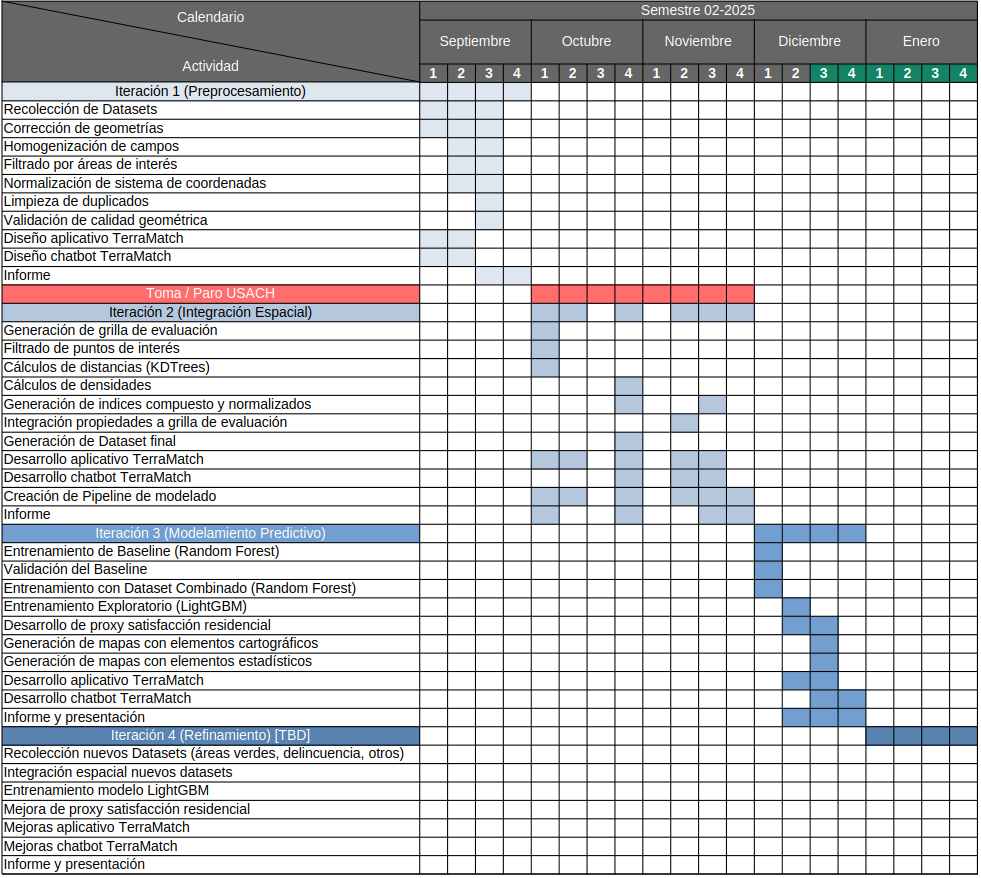
\includegraphics[width=0.9\textwidth]{figuras/figura3_carta_gant_sintetica.png}
    \caption{Carta Gantt sintética}
    \label{fig:carta_gantt}
\end{figure}

Se proyecta ejecutar estas tareas en enero 2026 por extension de semestre debido a toma/paro USACH, se priorizara validación con usuarios y mejoras en cobertura de datos.
\section{Conclusiones Preliminares}

El proyecto demuestra viabilidad tecnica y un enfoque replicable: la integracion de datos geoespaciales con ML permite explicar satisfaccion residencial con R\textsuperscript{2} > 0.86. Los resultados muestran que accesibilidad y entorno urbano complementan el precio en la explicacion de la satisfaccion, y que existen diferencias territoriales relevantes.

El enfoque integra datos heterogeneos en un pipeline reproducible y permite analizar accesibilidad urbana con un nivel de detalle espacial que no se obtiene solo con precios. Esto habilita comparaciones objetivas entre comunas y soporta recomendaciones personalizadas por perfil.

En terminos territoriales, el estudio evidencia un gradiente centro-periferia y diferencias marcadas entre comunas en transporte, salud y comercio. Estos hallazgos son coherentes con la estructura urbana de Santiago y refuerzan la utilidad de incluir variables geoespaciales en modelos inmobiliarios.

\subsection{Factibilidad, Desafios y Ajustes}
\begin{itemize}
    \item \textbf{Factibilidad:} datos y pipeline consolidados; metricas espaciales y modelo operativo.
    \item \textbf{Desafios:} variables no observadas (antiguedad, calidad, gastos) y temporalidad del mercado.
    \item \textbf{Ajustes propuestos:} ampliar cobertura comunal, incorporar variables ambientales/demograficas y validar con encuestas reales.
\end{itemize}

En conjunto, los resultados respaldan la continuidad del proyecto en una segunda fase con foco en validacion empirica, refinamiento de perfiles y despliegue de herramientas de apoyo a decision para usuarios finales.

\subsection{Proximos Pasos}
\begin{itemize}
    \item Implementar un prototipo de recomendacion y evaluacion con usuarios.
    \item Revisar bibliografia y fortalecer el marco teorico para la version final.
\end{itemize}

Finalmente, la version final incorporara bibliografia completa y validaciones adicionales con datos mas recientes, consolidando la utilidad del sistema para escenarios reales de decision.
\appendix
\section{Anexos}

\subsection{Anexo A: Código Adicional}

% Código extenso que no cabe en el cuerpo principal

\subsection{Anexo B: Tablas Complementarias}

\begin{table}[H]
\centering
\caption{Comunas alcance área de estudio}
\label{tab:comunas}
\begin{tabular}{@{}llll@{}}
\toprule
\textbf{Nombre Comuna} & \textbf{Coordenadas} & \textbf{Superficie total} & \textbf{Altura promedio}\\
\midrule 
Estación Central & $33^\circ 27' 07''\mathrm{S} \quad 70^\circ 40' 44''\mathrm{O}$ & 14.1 km² & 512 m\\
La Reina &  $33^\circ 27' 00''\mathrm{S} \quad 70^\circ 33' 00''\mathrm{O}$ & 23.4 km² & 680 m\\
Ñuñoa &  $33^\circ 28' 00''\mathrm{S} \quad 70^\circ 36' 00''\mathrm{O}$ & 16.9 km² & 560 m\\
Santiago Centro &  $33^\circ 27' 00''\mathrm{S} \quad 70^\circ 40' 00''\mathrm{O}$ & 22.4 km² & 520 m\\
\bottomrule
\end{tabular}
\end{table}

\begin{table}[H]
\centering
\caption{Resumen de fuentes de datos utilizadas}
\label{tab:datos}
\begin{tabular}{@{}llllll@{}}
\toprule
\textbf{Dato} & \textbf{Fuente} & \textbf{Formato} & \textbf{Resolución} & \textbf{Fecha} & \textbf{Acceso} \\
\midrule
Buffer La Reina & GoogleMaps & .geojson & Poligono & 2025 & GoogleMaps API \\
Buffer Est. Central & GoogleMaps & .geojson & Poligono & 2025 & GoogleMaps API \\
Buffer Ñuñoa & GoogleMaps & .geojson & Poligono & 2025 & GoogleMaps API \\
Buffer Stgo. Centro & GoogleMaps & .geojson & Poligono & 2025 & GoogleMaps API \\
Ubic. Casas La Reina & GoogleMaps & .geojson & Punto & 2025 & GoogleMaps API \\
Ubic. Casas Est. Central & GoogleMaps & .geojson & Punto & 2025 & GoogleMaps API \\
Ubic. Casas Ñuñoa & GoogleMaps & .geojson & Punto & 2025 & GoogleMaps API \\
Ubic. Casas Stgo. Centro & GoogleMaps & .geojson & Punto & 2025 & GoogleMaps API \\
Descrip. Casas La Reina & PortalInmobiliario & .csv & Punto & 2025 & Scraping \\
Descrip. Casas Est. Central & PortalInmobiliario & .csv & Punto & 2025 & Scraping \\
Descrip. Casas Ñuñoa & PortalInmobiliario & .csv & Punto & 2025 & Scraping \\
Descrip. Casas Stgo. Centro & PortalInmobiliario & .csv & Punto & 2025 & Scraping \\
Ubic. Deptos La Reina & GoogleMaps & .geojson & Punto & 2025 & GoogleMaps API \\
Ubic. Deptos Est. Central & GoogleMaps & .geojson & Punto & 2025 & GoogleMaps API \\
Ubic. Deptos Ñuñoa & GoogleMaps & .geojson & Punto & 2025 & GoogleMaps API \\
Ubic. Deptos Stgo. Centro & GoogleMaps & .geojson & Punto & 2025 & GoogleMaps API \\
Descrip. Deptos La Reina & PortalInmobiliario & .csv & Punto & 2025 & Scraping \\
Descrip. Deptos Est. Central & PortalInmobiliario & .csv & Punto & 2025 & Scraping \\
Descrip. Deptos Ñuñoa & PortalInmobiliario & .csv & Punto & 2025 & Scraping \\
Descrip. Deptos Stgo. Centro & PortalInmobiliario & .csv & Punto & 2025 & Scraping \\
Censo & INE Chile & .csv & Manzana & 2017 & Portal INE \\
\bottomrule
\end{tabular}
\end{table}

\subsection{Anexo C: Figuras y Graficos}

\begin{figure}[H]
    \centering
    % \includegraphics[width=\textwidth]{figuras/diagrama_flujo.png}
    \caption{Diagrama de flujo metodológico del proyecto}
    \label{fig:flujo}
\end{figure}

\begin{figure}[H]
    \centering
    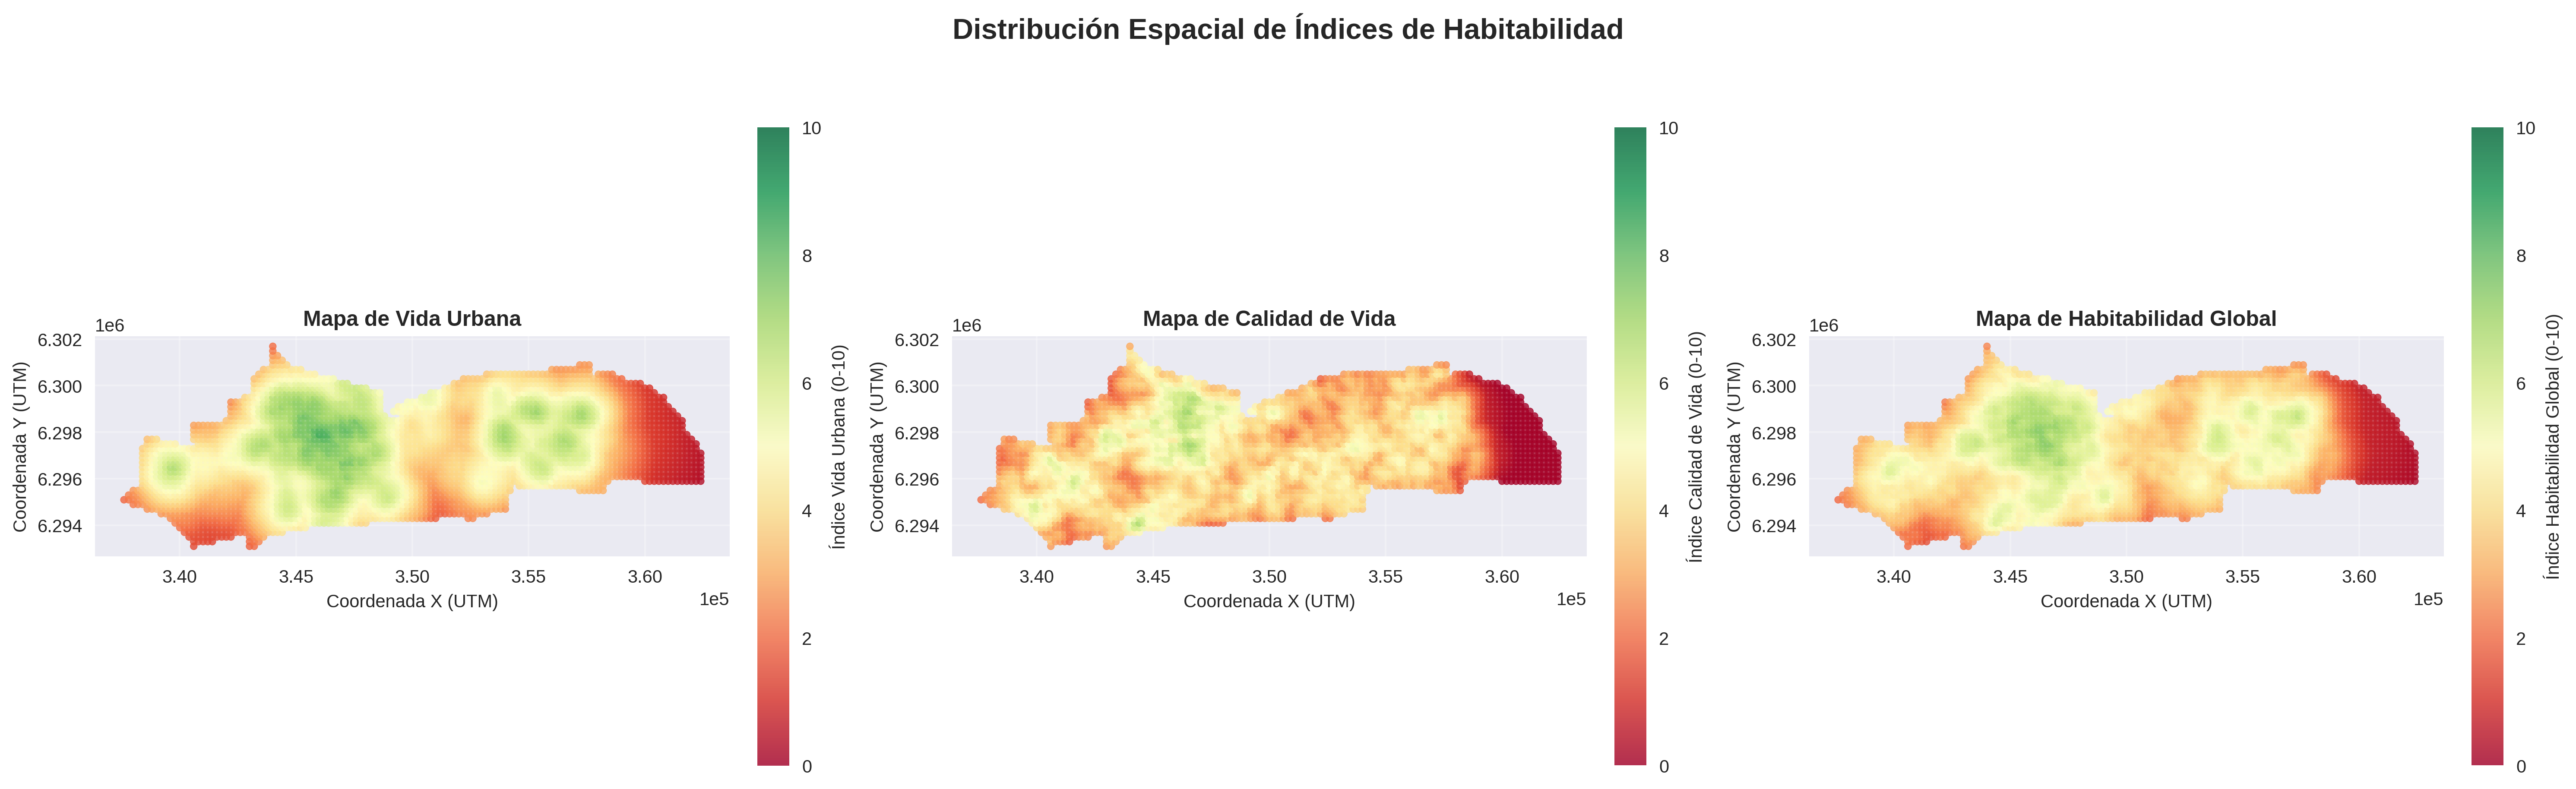
\includegraphics[width=0.75\textwidth]{figuras/05_mapa_habitabilidad.png}
    \caption{Mapa de índice de habitabilidad calculado a partir de características espaciales}
    \label{fig:mapa_habitabilidad}
\end{figure}

\begin{figure}[H]
    \centering
    
\includegraphics[width=0.9\textwidth]{figuras/grafico_01_histogramas.png}
    \caption{Distribución de variables principales: precio (UF), superficie útil (m²), dormitorios y baños}
    \label{fig:histogramas}
\end{figure}

\begin{figure}[H]
    \centering
    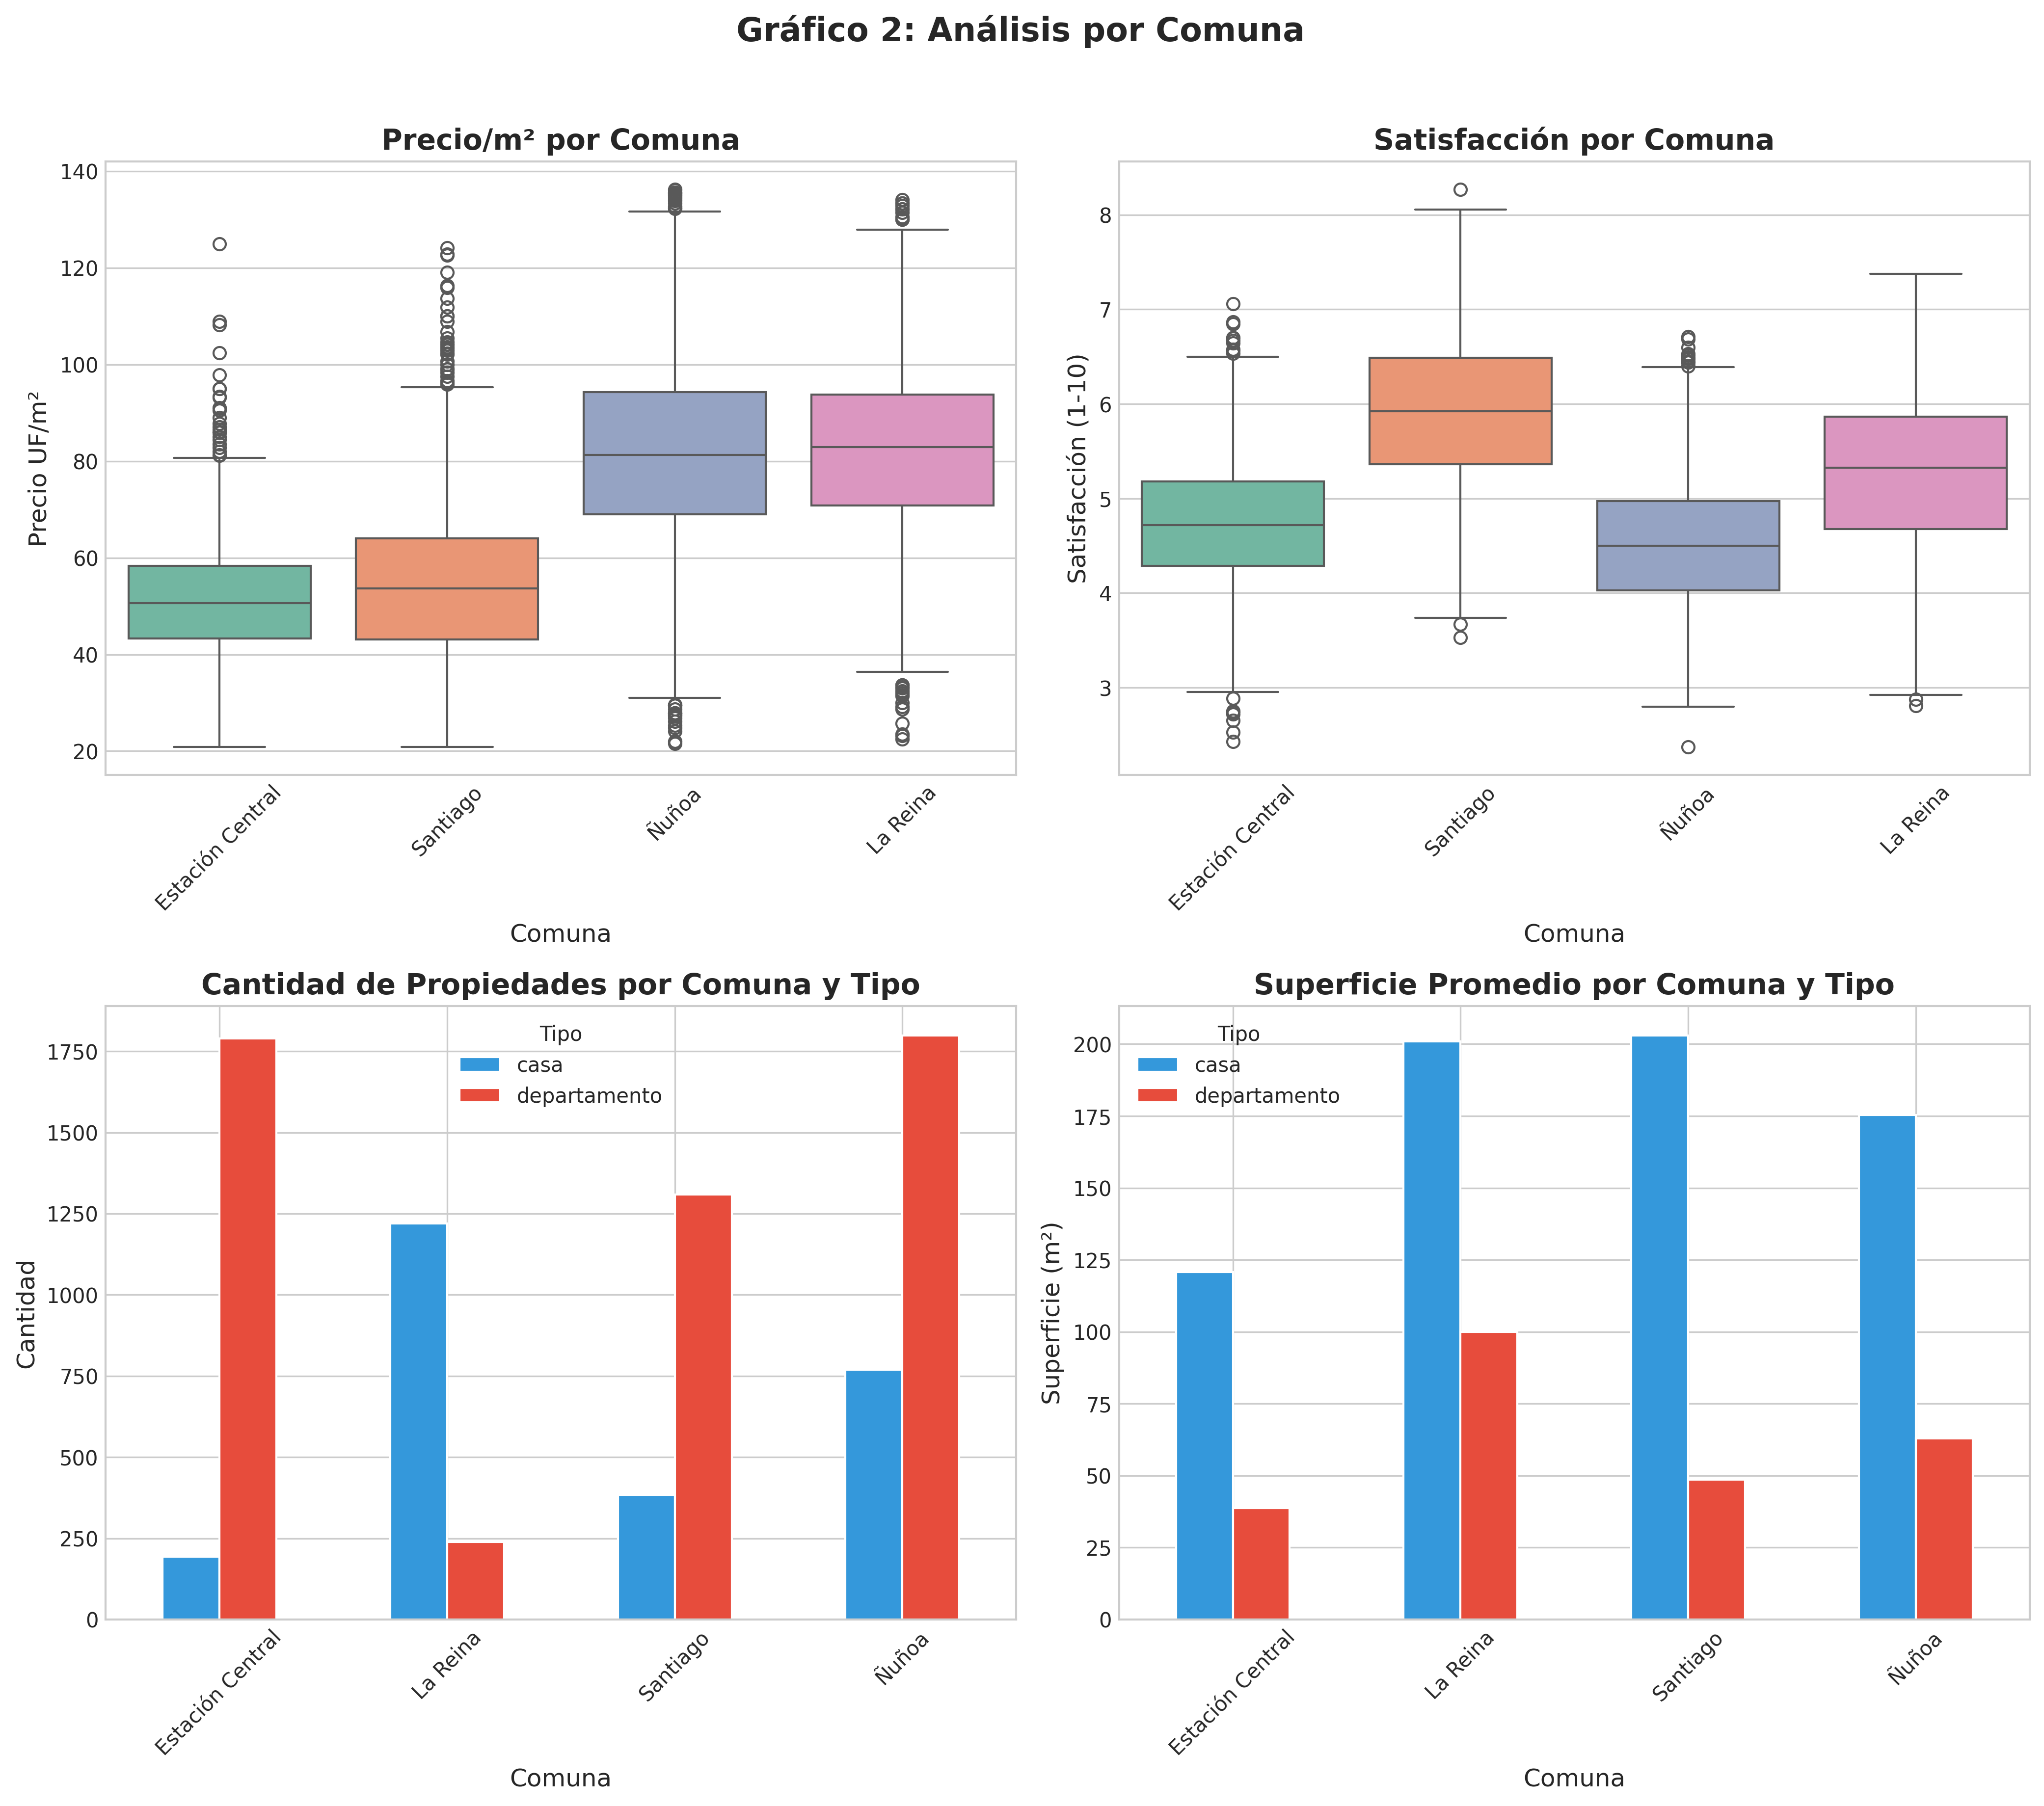
\includegraphics[width=0.95\textwidth]{figuras/grafico_02_analisis_comunas.png}
    \caption{Análisis comparativo de propiedades por comuna: distribución de precios, superficies y características}
    \label{fig:analisis_comunas}
\end{figure}

\begin{figure}[H]
    \centering
    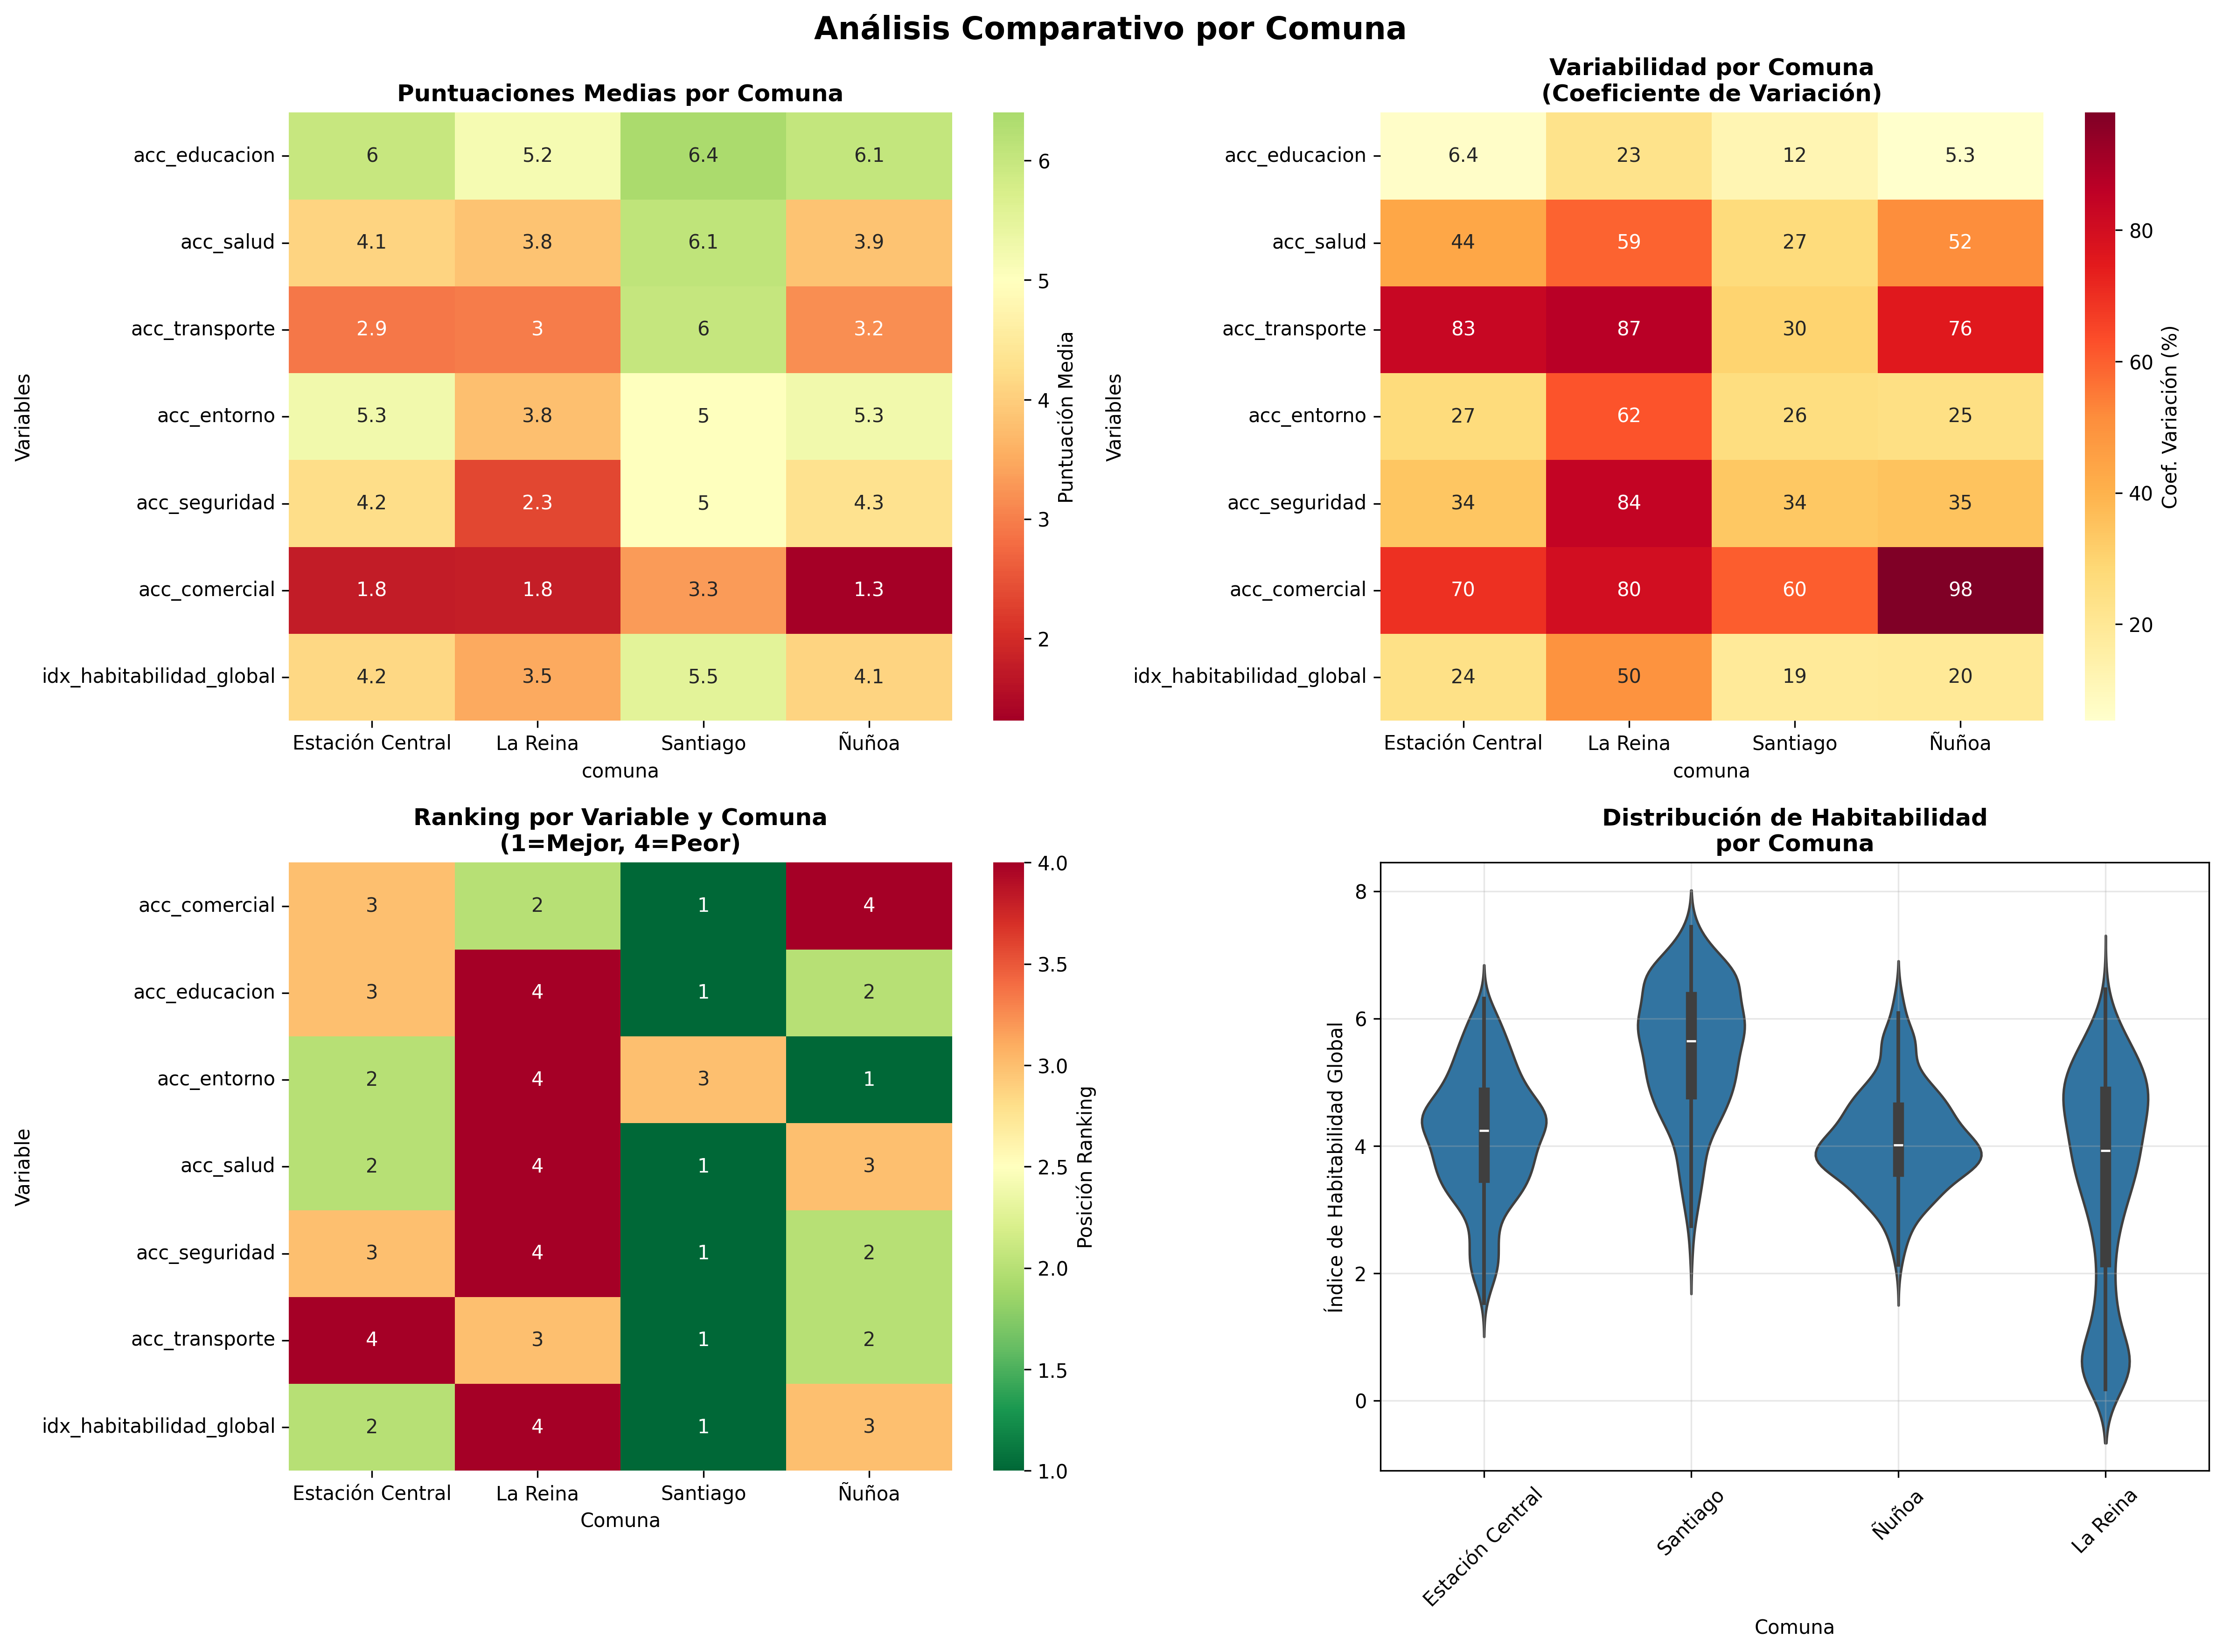
\includegraphics[width=0.9\textwidth]{figuras/10_analisis_por_comuna.png}
    \caption{Análisis detallado de características espaciales por comuna}
    \label{fig:detalle_comunas}
\end{figure}

\begin{figure}[H]
    \centering
    
\includegraphics[width=0.9\textwidth]{figuras/mapa_02_precio_m2.png}
    \caption{Distribución espacial del precio por metro cuadrado (UF/m²) en las 4 comunas}
    \label{fig:mapa_precios}
\end{figure}

\begin{figure}[H]
    \centering
    
\includegraphics[width=0.85\textwidth]{figuras/grafico_03_correlaciones.png}
    \caption{Matriz de correlaciones entre variables de propiedades y características espaciales}
    \label{fig:correlaciones}
\end{figure}

\begin{figure}[H]
    \centering
    
\includegraphics[width=0.9\textwidth]{figuras/mapa_03_satisfaccion_predicha.png}
    \caption{Mapa de satisfacción residencial predicha: visualización estática de la distribución espacial de predicciones del modelo LightGBM en las 4 comunas}
    \label{fig:mapa_satisfaccion}
\end{figure}

\begin{figure}[H]
    \centering
    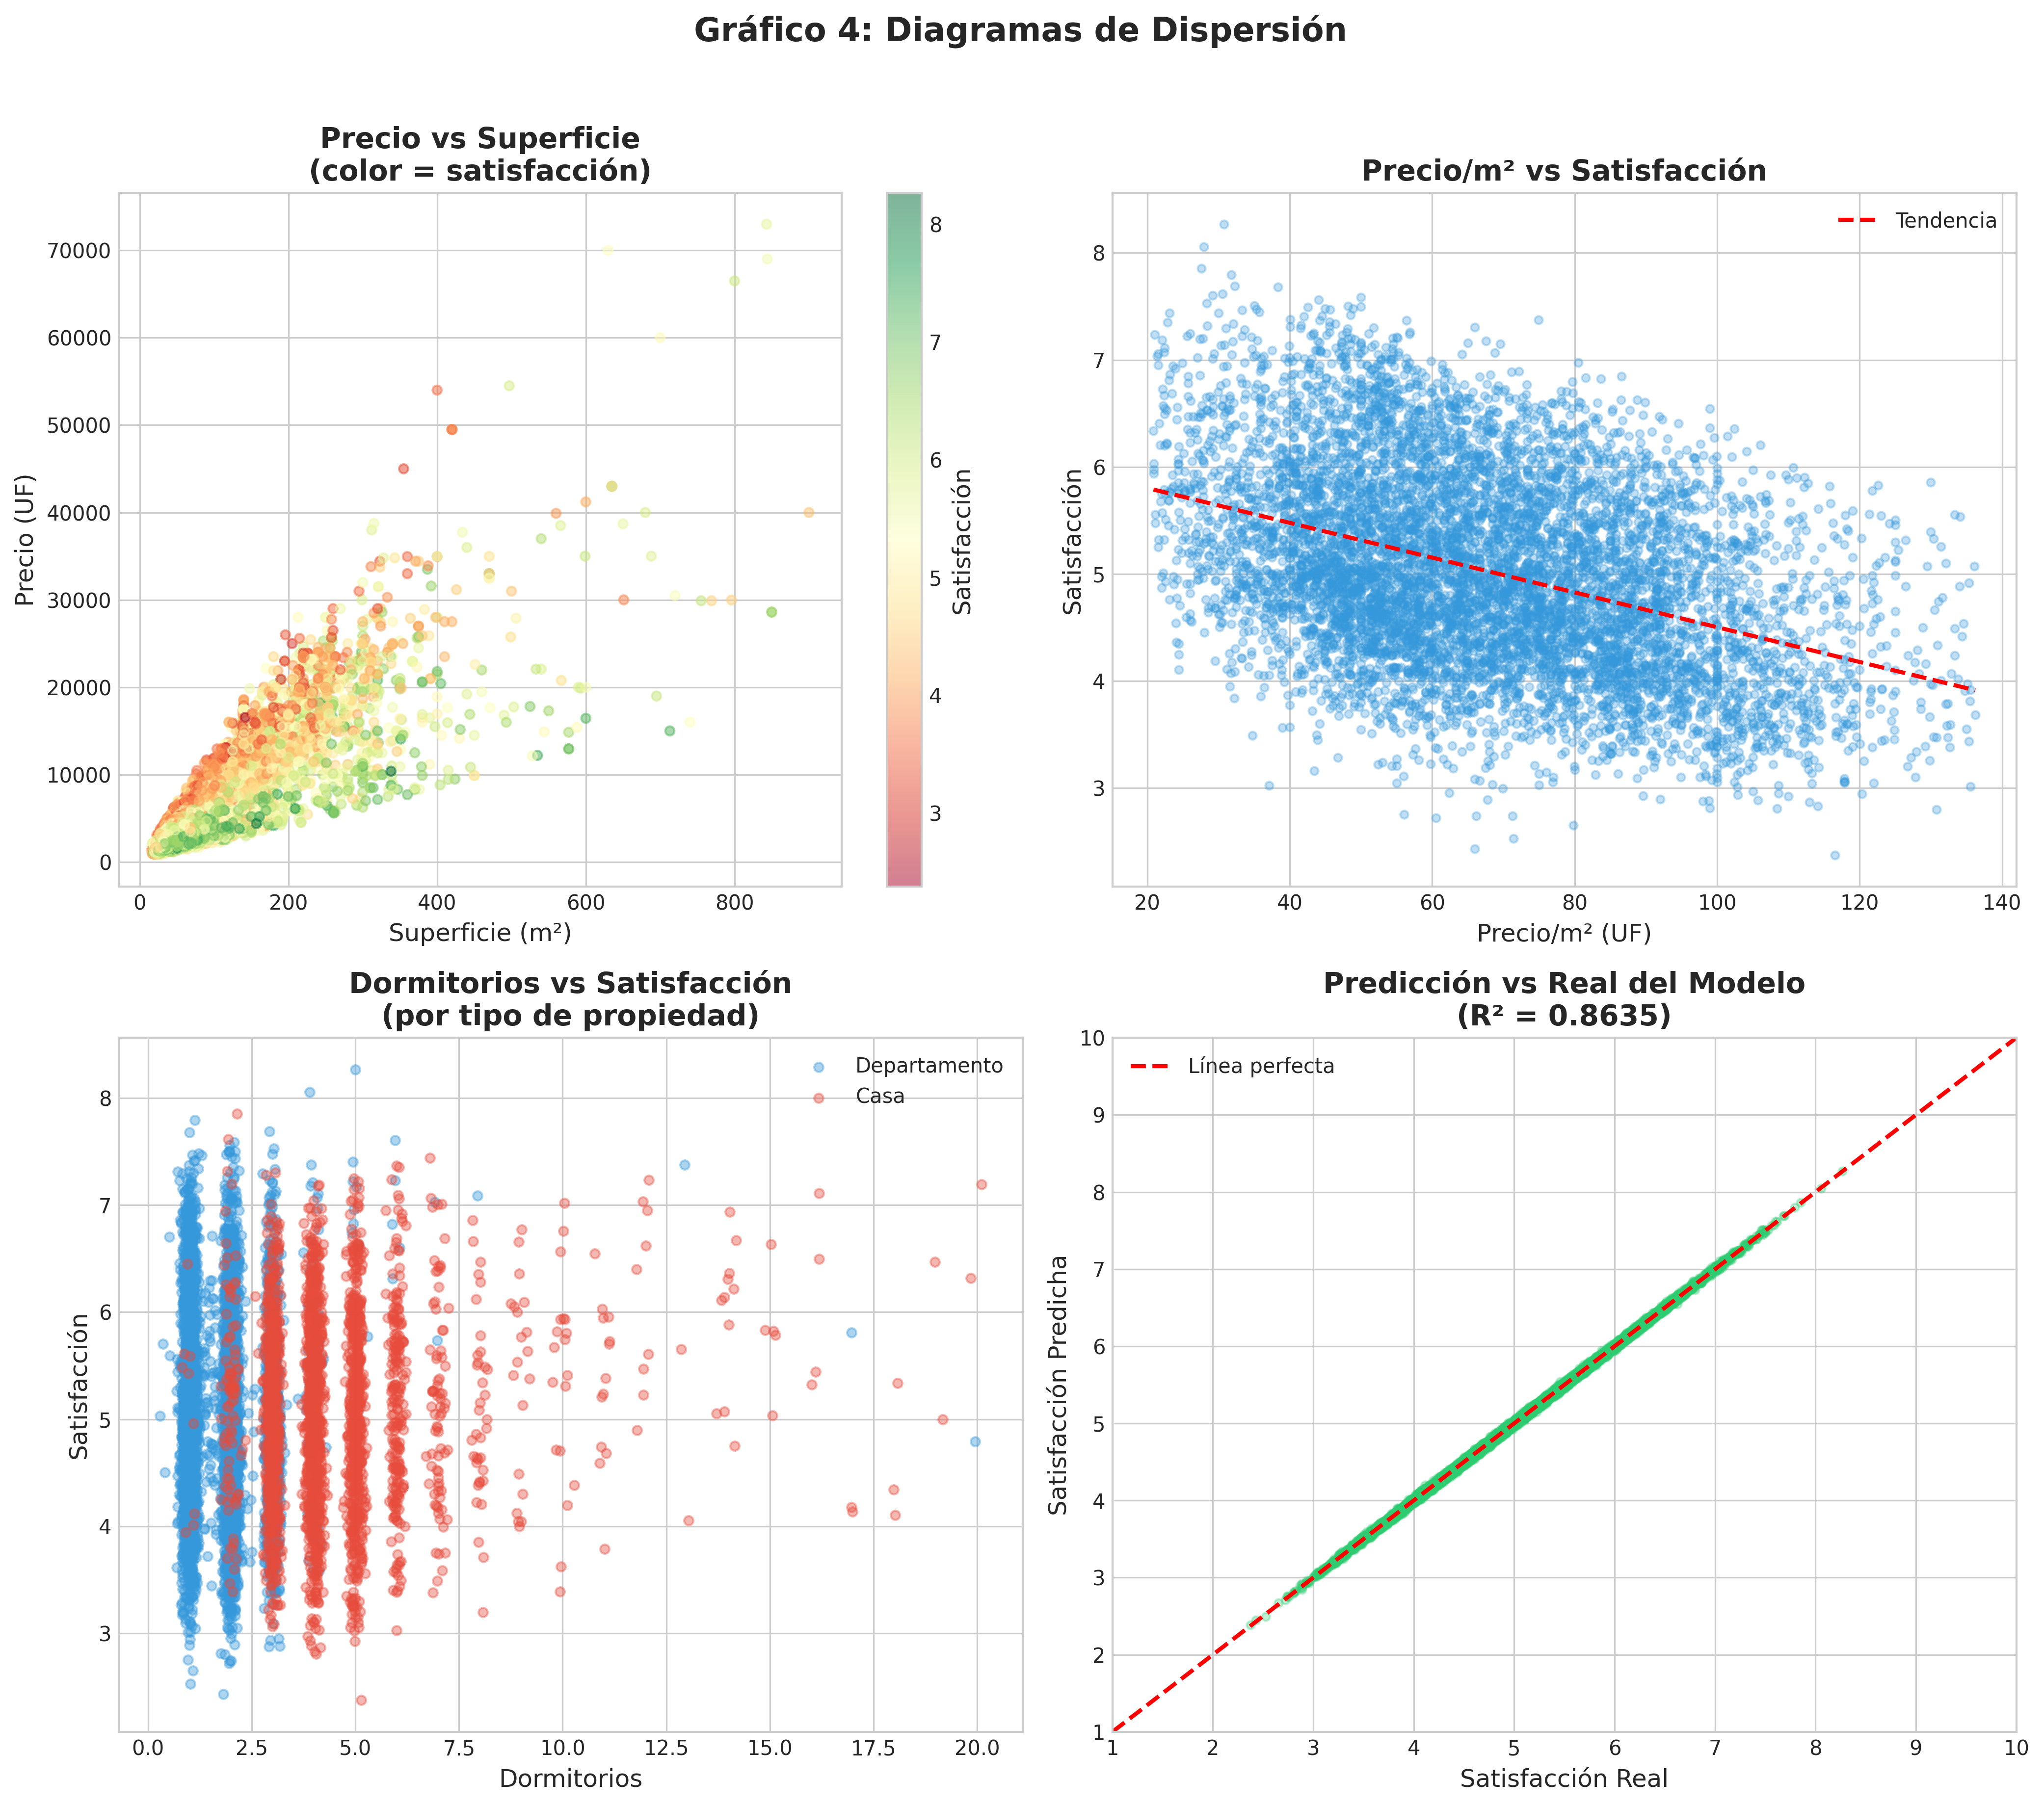
\includegraphics[width=0.8\textwidth]{figuras/grafico_04_dispersion.png}
    \caption{Gráfico de dispersión: satisfacción predicha vs. satisfacción real (R² = 0.8635)}
    \label{fig:dispersion}
\end{figure}

\begin{figure}[H]
    \centering
    
\includegraphics[width=0.9\textwidth]{figuras/grafico_05_importancia_metricas.png}
    \caption{Importancia de las 20 principales variables en el modelo predictivo LightGBM}
    \label{fig:importancia}
\end{figure}

\begin{figure}[H]
    \centering
    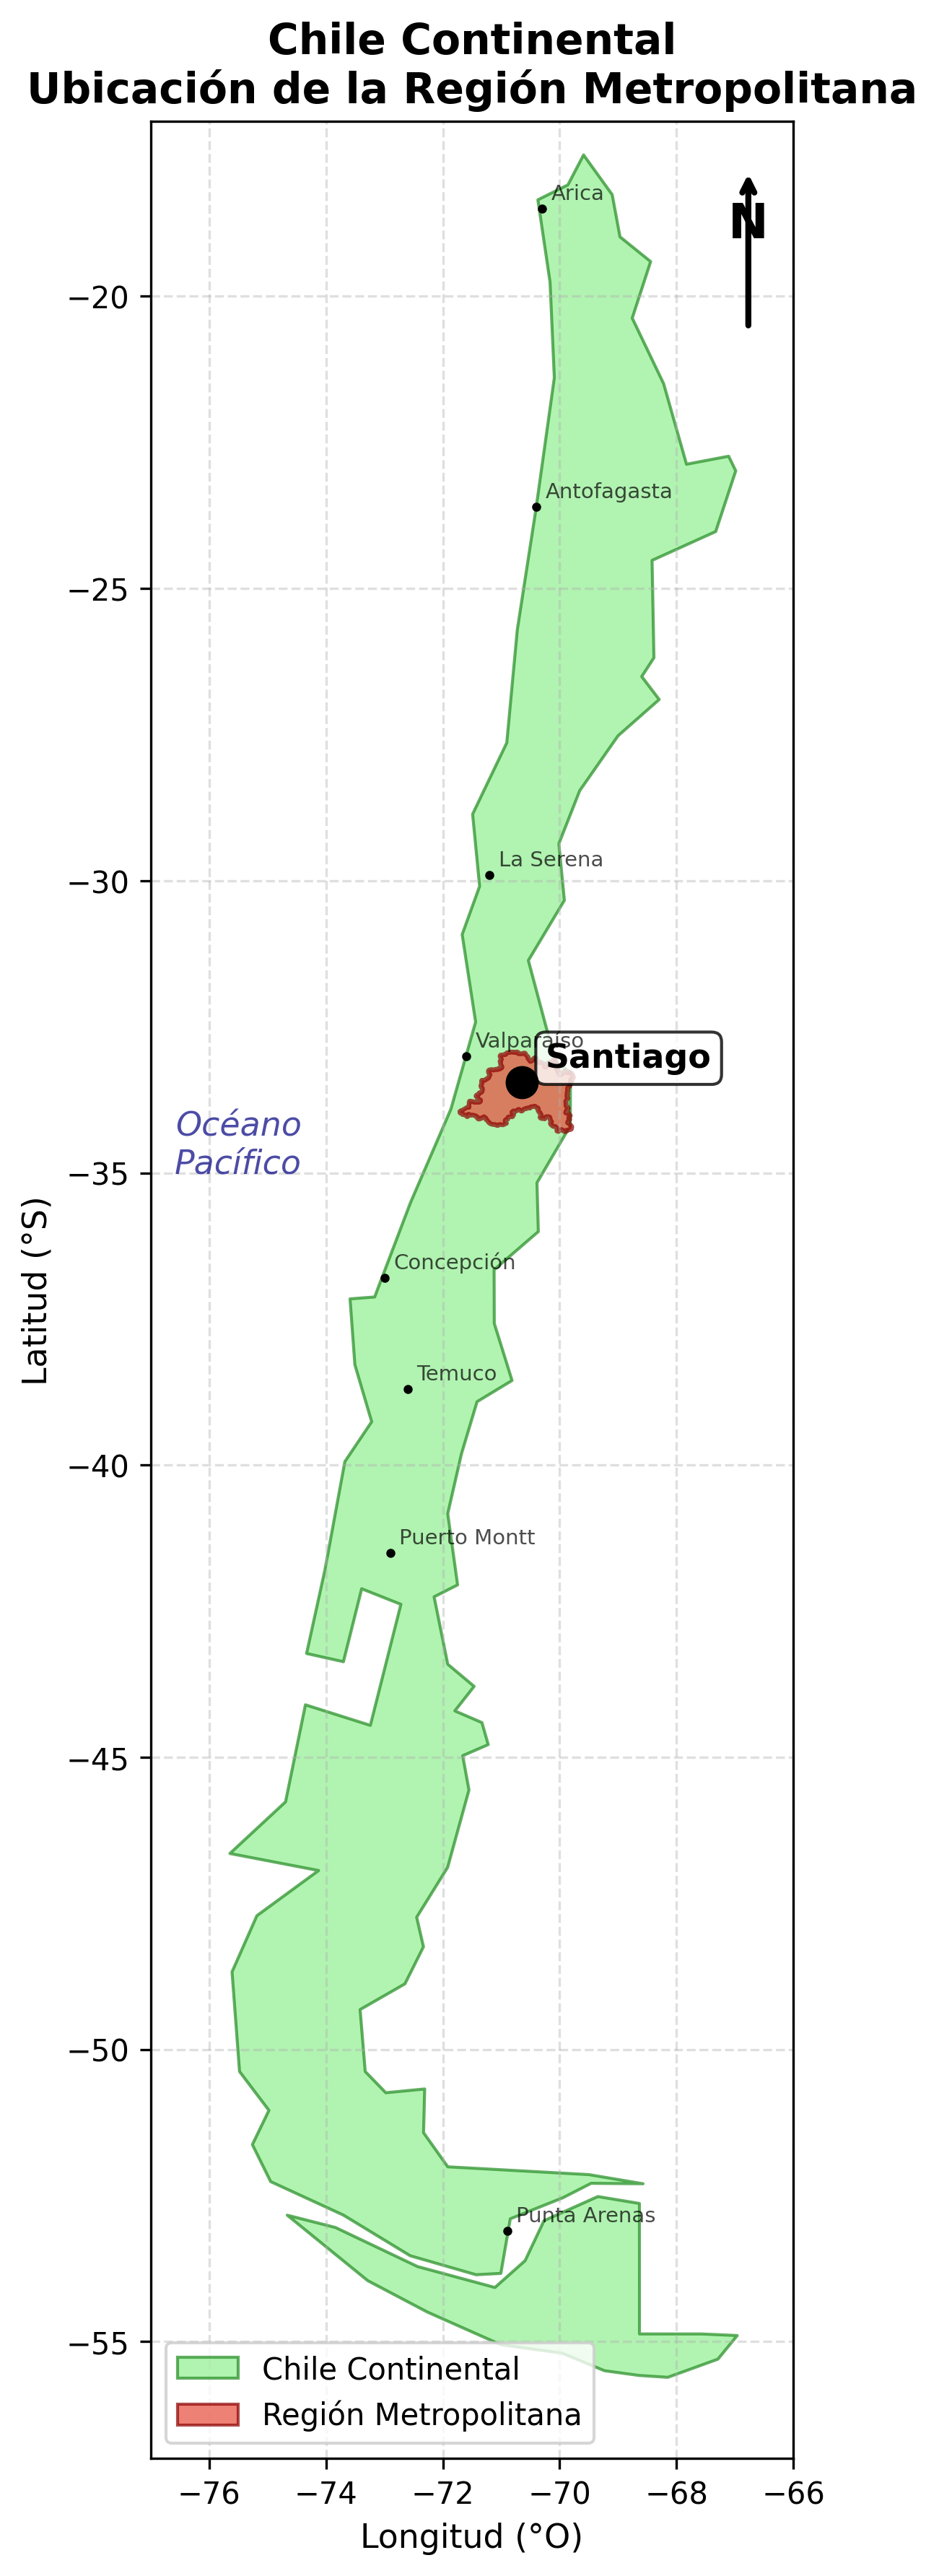
\includegraphics[width=0.4\textwidth]{figuras/figura1_chile_rm.png}
    \caption{Mapa ubicación Región Metropolitana de Santiago}
    \label{fig:ubicacion}
\end{figure}

\begin{figure}[H]
    \centering
    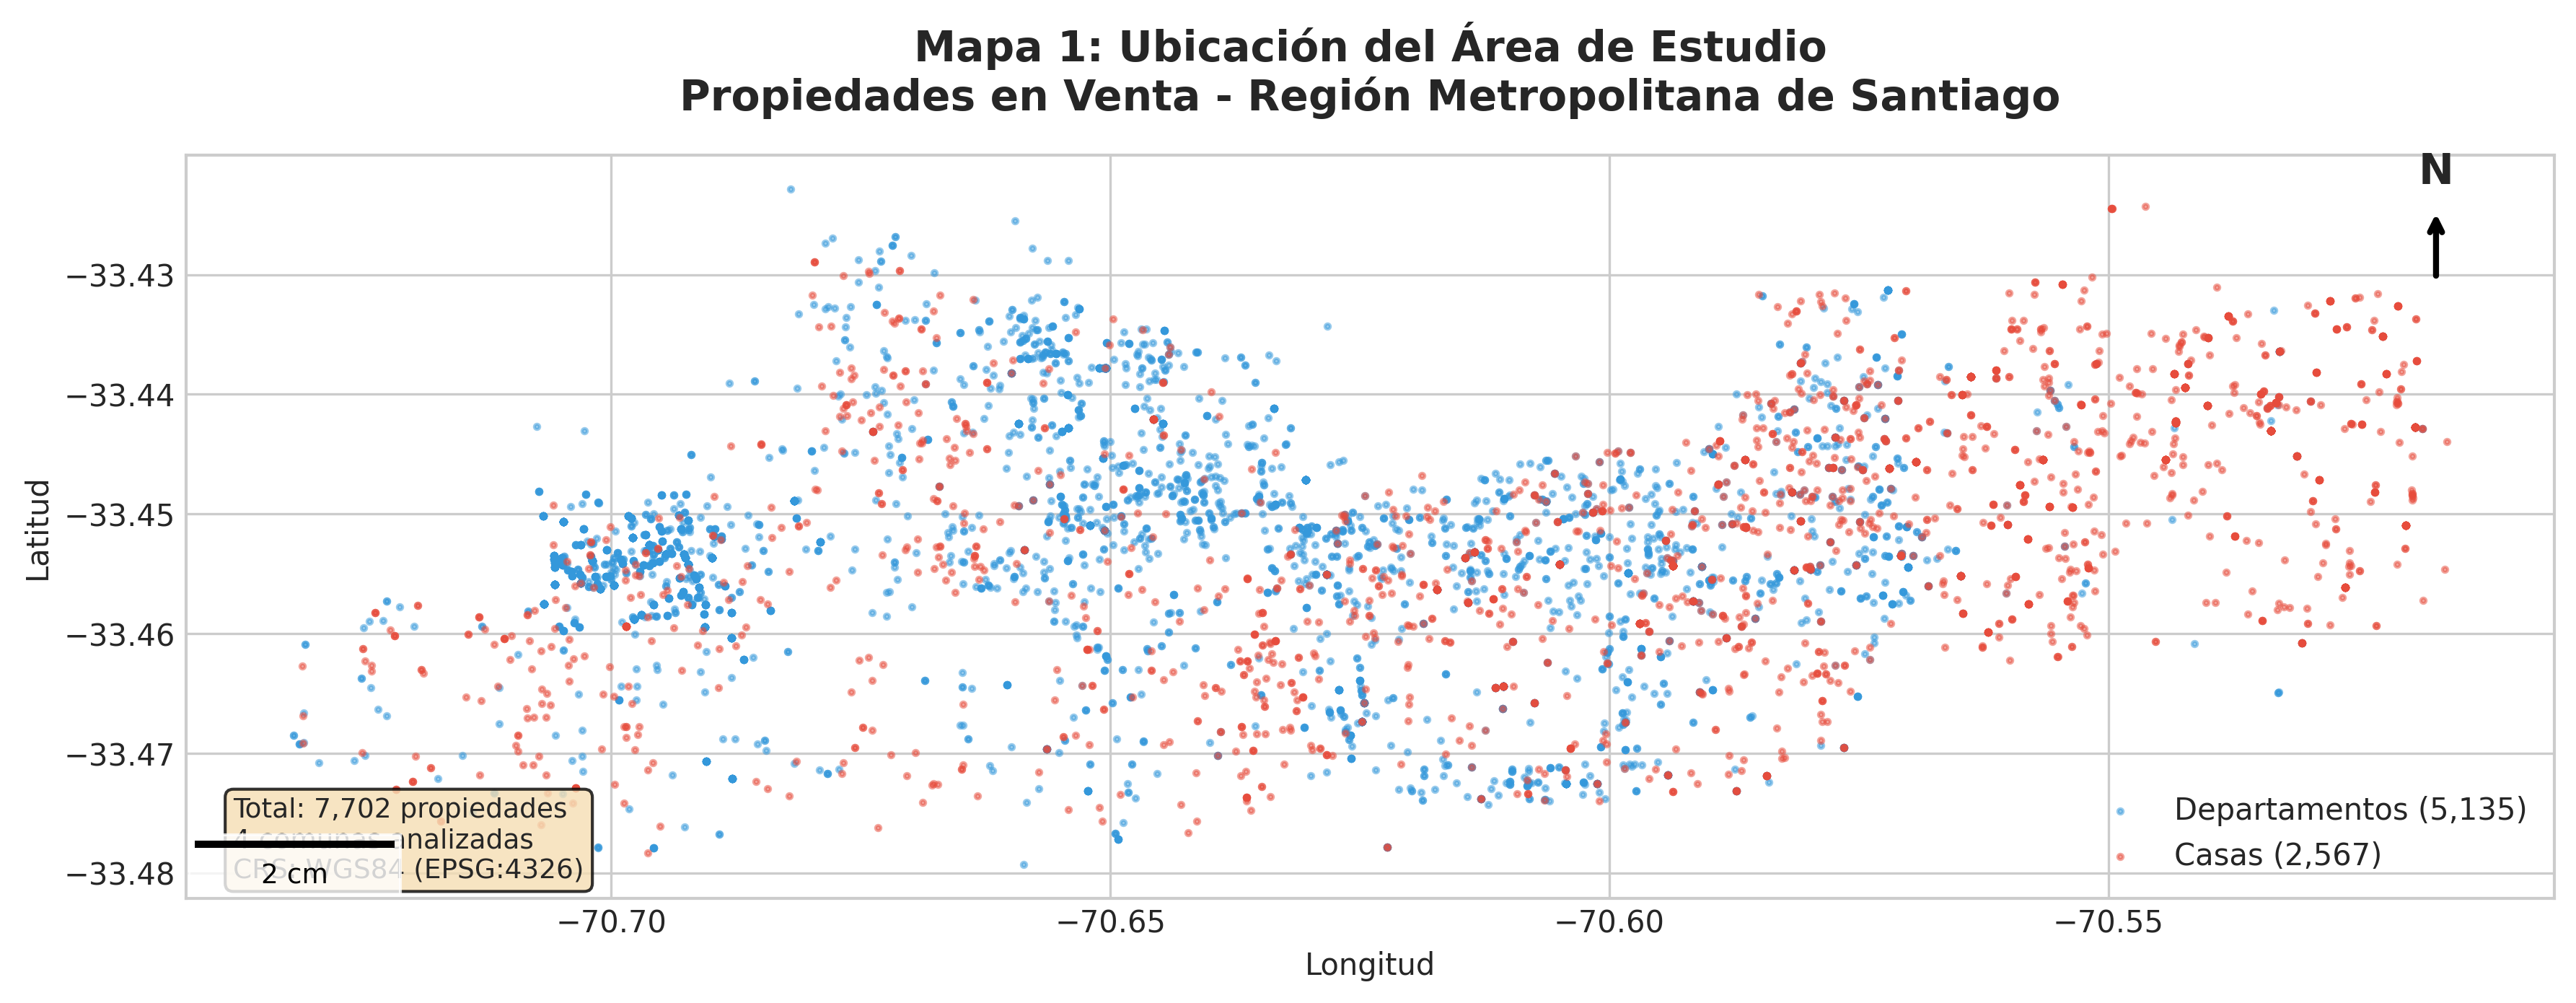
\includegraphics[width=0.8\textwidth]{figuras/mapa_01_ubicacion_area_estudio.png}
    \caption{Mapa de ubicación del área de estudio (4 comunas: Estación Central, La Reina, Ñuñoa y Santiago Centro)}
    \label{fig:ubicacion_area}
\end{figure}
\subsection{Anexo D: Enlaces y Recursos}

\begin{itemize}
    \item \textbf{Repositorio GitHub:} \url{https://github.com/usuario/proyecto}
    \item \textbf{Dashboard interactivo:} \url{http://link-al-dashboard}
    \item \textbf{Datos originales:} \url{http://link-a-datos}
\end{itemize}

\end{document}
